\chapter{Dictionnaires}
\label{chap-dictionaries}

\section{Les dictionnaires DELA}
\index{DELA}\index{Dictionnaire!format}\index{LADL}

Les dictionnaires électroniques utilisés par Unitex utilisent le formalisme DELA (Dictionnaires
Electroniques du LADL). Ce formalisme permet de décrire les entrées lexicales simples et composées
\index{Entrée lexicale} d’une langue en leur associant de façon optionnelle des
informations grammaticales, sémantiques et flexionnelles. On distingue deux sortes de dictionnaires
électroniques. Le type que l’on utilise le plus couramment est le dictionnaire de formes fléchies,
appelé DELAF (DELA de formes Fléchies) ou encore DELACF (DELA de formes Composées
Fléchies) lorsqu’il s’agit d’un dictionnaire de mots composés.\index{DELAF|(}
\index{DELACF}\index{Dictionnaire!DELAF|(}\index{Dictionnaire!DELACF}
Le second type est le dictionnaire de formes non fléchies appelé DELAS (DELA de formes Simples)
ou DELAC (DELA de formes Composées).
\index{DELAS}\index{DELAC}\index{Dictionnaire!DELAS}\index{Dictionnaire!DELAC}
Les programmes d’Unitex ne font pas de distinction entre les dictionnaires de formes
simples et composées. Nous utiliserons donc les termes DELAF et DELAS pour désigner les deux sortes
de dictionnaires que leurs entrées soient simples, composées ou mixtes.

\subsection{Format des DELAF}
\label{section-DELAF-format}
\subsubsection{Syntaxe d’une entrée}
\label{section-DELAF-entry-syntax}
Une entrée d’un DELAF est une ligne de texte terminée par un retour à la ligne qui
respecte le schéma suivant :

\bigskip
\begin{verbatim}
mercantiles,mercantile.A+z1:mp:fp/ceci est un exemple
\end{verbatim}

\bigskip
\noindent Les différents éléments qui forment cette ligne sont les suivants:

\bigskip
\begin{itemize}
\item \verb+mercantiles + est la forme fléchie de l’entrée.\index{Forme!fléchie} Cette forme fléchie
est obligatoire;
  
\bigskip \item \verb+mercantile+ est la forme canonique (lemme) de l’entrée.
\index{Lemme}\index{Forme!canonique} Pour les noms et les adjectifs, il s’agit
en général de la forme au masculin singulier; pour les verbes, la forme canonique est
l’infinitif. Cette information peut être omise comme dans l’exemple suivant :

  
\bigskip
\verb$boîte à merveilles,.N+z1:fs$
  
\bigskip Cela signifie alors que la forme canonique est identique à la forme fléchie. La forme
canonique est séparée de la forme fléchie par une virgule;
\index{\verbc{,}}
  
\bigskip \item \verb$A+z1$ est la séquence d’informations grammaticales et sémantiques.
\index{Informations!grammaticales}\index{Informations!sémantiques} Dans notre exemple, \verb+A+
désigne un adjectif, et \verb+z1+ ndique qu’il s’agit d’un mot courant (voir tableau ~\ref{tab-semantic-codes}).

Toute entrée doit comporter au moins un code grammatical ou sémantique, séparé de
la forme canonique par un point. S’il y a plusieurs codes, ceux-ci doivent être séparés
par le caractère \verb$+$\index{\verbc{+}}\index{\verbc{.}}.
  
\bigskip
\item \verb+:mp:fp+ est la séquence d’informations flexionnelles.
\index{Informations!flexionnelles} Ces informations décrivent le genre, le nombre, les temps et modes
de conjugaisons, les déclinaisons pour les langues à cas, etc. Ces informations sont facultatives.
Un code flexionnel est composé d’un ou plusieurs caractères codant chacun une information. Les codes
flexionnels doivent être séparés par le caractère :. Dans notre exemple, \verb+m+ signifie masculin,
\verb+p+ pluriel et \verb+f+ féminin (voir tableau ~\ref{tab-inflectional-codes}). Le caractère \verb+:+ s’interprète comme un OU logique. Ainsi, \verb+:mp:fp+ signifie "masculin pluriel", ou "féminin pluriel". Comme chaque caractère correspond à une information, il est inutile d’utiliser plusieurs fois un même caractère. Ainsi, coder le participe passé avec le code\verb+:PP+ serait strictement équivalent à utiliser \verb+:P+ seul;\index{\verbc{:}}
  
\bigskip \item \verb+/ceci est un exemple+ est un commentaire. Les commentaires sont facultatifs et
doivent être introduits par le caractère \verb+/+. Les commentaires sont supprimés lorsque
l’on comprime les dictionnaires. \index{Commentaire!dans un dictionnaire} \index{Dictionnaire!commentaire}\index{\verbc{/}}
\end{itemize}

\bigskip
\noindent REMARQUE IMPORTANTE : il est possible d’utiliser le point et la virgule dans une
entrée de dictionnaire. Pour cela, il faut les déspécialiser avec le caractère
\verb+\+ \index{\verbt{\textbackslash,}}\index{\verbt{\textbackslash.}}\index{\verbt{\textbackslash~}}:

\bigskip
\begin{verbatim}
3\,1415,PI.NOMBRE
Organisation des Nations Unies,O\.N\.U\..SIGLE
\end{verbatim}


\bigskip
\noindent ATTENTION : chaque caractère est pris en compte dans une ligne de dictionnaire. Par
exemple, si vous introduisez des espaces, ceux-ci seront considérés comme faisant partie
intégrante des informations. Dans la ligne suivante :


\begin{verbatim}
gît,gésir.V+z1:P3s /voir ci-gît
\end{verbatim}

\bigskip \noindent l’espace qui précède le caractère \verb+/+ sera considéré comme faisant partie
d’un code flexionnel à 4 caractères composés de \verb+P+, \verb+3+, \verb+s+ et d’un espace.


\bigskip \noindent Il est possible d’insérer des lignes de commentaires dans un dictionnaire DELAF
ou DELAS, en faisant débuter la ligne par le caractère $/$. Exemple

\bigskip
\begin{verbatim}
/ L’entrée nominale pour ’par’ est un terme de golf
par,.N+z3:ms
\end{verbatim}


\subsubsection{Mots composés avec espace ou tiret}

\index{Mots!composés!avec espace ou tiret}\index{\verbc{=}}\index{\verbt{\textbackslash=}}

Certains mots composés comme \textit{grand-mère} peuvent s’écrire avec des espaces ou avec
des tirets. Pour éviter de devoir dédoubler toutes les entrées, il est possible d’utiliser 
le caractère \verb+=+ . Lors de la compression du dictionnaire, le programme \verb+Compress+
\index{Programmes externes!\verbc{Compress}}\index{\verbc{Compress}} vérifie pour chaque ligne
si la forme fléchie ou la forme canonique contient le caractère \verb+=+. Si c’est le cas, le
programme remplace l’entrée par deux entrées : une où le caractère = est remplacé par un espace,
et une où il est remplacé par un tiret. Ainsi, l’entrée suivante :


\bigskip \verb$grand=mères,grand=mère.N:fp$

\bigskip
\noindent est remplacée par les deux lignes suivantes:

\bigskip
\verb$grand mères,grand mère.N:fp$

\verb$grand-mères,grand-mère.N:fp$


\bigskip
\noindent NOTE : si vous souhaitez écrire une entrée contenant le caractère \verb+=+,
déspécialisez-le avec le caractère \verb+\+ comme dans l’exemple suivant :


\bigskip
\verb$E\=mc2,.FORMULE$\\


Cette opération de remplacement a lieu lors de la compression du dictionnaire. Une fois
le dictionnaire comprimé, les signes \verb+=+ déspécialisés sont remplacés par de simples \verb+=+.
Ainsi, si l’on comprime un dictionnaire contenant les lignes suivantes :


\begin{verbatim}
E=mc2,.FORMULE
grand=mère,.N:fs
\end{verbatim}

\noindent et que l’on applique ce dictionnaire au texte :\\

\verb$Ma grand-mère m’a expliqué la formule E=mc2.$


\bigskip \noindent on obtiendra les lignes suivantes dans le dictionnaire de mots composés du texte:


\begin{verbatim}
E=mc2,.FORMULE
grand-mère,.N:fs
\end{verbatim}


\subsubsection{Factorisation d’entrées}

Plusieurs entrées ayant les mêmes formes fléchie et canonique peuvent être regroupées
en une seule à condition qu’elle aient les mêmes codes grammaticaux et sémantiques. Cela
permet entre autres de regrouper des conjugaisons identiques pour un même verbe :


\bigskip
\begin{verbatim}
glace,glacer.V+z1:P1s:P3s:S1s:S3s:Y2s
\end{verbatim}

\bigskip 
\noindent Si les informations grammaticales et sémantiques diffèrent, il faut créer des entrées dis-
tinctes :


\bigskip
\begin{verbatim}
glace,.N+z1:fs
glace,glacer.V+z1:P1s:P3s:S1s:S3s:Y2s
\end{verbatim}

\bigskip 
\noindent Certaines entrées ayant les mêmes codes grammaticaux et sémantiques peuvent avoir
des sens différents, comme c’est le cas pour le mot \textit{poêle} qui désigne un appareil de
chauffage ou un voile au masculin et un instrument de cuisine au féminin. On peut donc distinguer
les entrées dans ce cas :


\bigskip
\noindent
\texttt{poêle,.N+z1:fs/ poêle à frire}

\noindent
\texttt{poêle,.N+z1:ms/ voile, linceul; appareil de chauffage}

\bigskip 
\noindent NOTE : dans la pratique, cette distinction n’a pas d’autre conséquence qu’une
augmentation du nombre d’entrées du dictionnaire. Les différents programmes qui composent Unitex
donneront exactement les mêmes résultats si l’on fusionne ces entrées en :

\bigskip
\noindent
\texttt{poêle,.N+z1:fs:ms}

\bigskip 
\noindent L’intérêt de cette distinction est donc laissé à l’appréciation des personnes qui
construisent des dictionnaires.


\index{DELAF|)}\index{Dictionnaire!DELAF|)}

\subsection{Format des DELAS}
\label{section-DELAS-format}
\index{DELAS}\index{Dictionnaire!DELAS}

Le format des DELAS est très similaire à celui des DELAF. La différence est qu’on ne
mentionne qu’une forme canonique suivie de codes grammaticaux et/ou sémantiques. La
forme canonique est séparée des différents codes par une virgule. Voici un exemple d’entrée :


\begin{verbatim}
cheval,N4+Anl
\end{verbatim}

\noindent Le premier code grammatical ou sémantique sera interprété par le programme de flexion
comme le nom de la grammaire à utiliser pour fléchir l’entrée. L’entrée de l’exemple cidessus
indique que le mot \textit{cheval} doit être fléchi avec une grammaire nommée \verb+N4+.
Il est possible d’ajouter des codes flexionnels aux entrées, mais la nature de l’opération de
flexion limite l’intérêt de cette possibilité. Pour plus de détails, voir plus loin dans ce chapitre
la section ~\ref{section-automatic-inflection}.


\subsection{Contenu des dictionnaires}
\index{Dictionnaire!contenu}\index{Dictionnaire!codes utilisés}

Les dictionnaires fournis avec Unitex contiennent des descriptions des mots simples et
composés. Ces descriptions indiquent la catégorie grammaticale de chaque entrée, ses 
éventuels codes de flexion, ainsi que des informations sémantiques diverses. Les tableaux 
suivants donnent un aperçu des différents codes utilisés dans les dictionnaires fournis avec
Unitex. Ces codes ont la même signification pour presque toutes les langues, même si certains
d’entre eux sont propres à certaines langues (\textit{i.e.} marque du neutre, etc.).

\begin{table}[!ht]
\index{\verbc{A}}\index{\verbc{ADV}}\index{\verbc{CONJC}}\index{\verbc{CONJS}}\index{\verbc{DET}}
\index{\verbc{INTJ}}\index{\verbc{N}}\index{\verbc{PREP}}\index{\verbc{PRO}}\index{\verbc{V}}
\begin{center}
\begin{tabular}{|c|l|l|}
\hline
\textbf{Code} & \textbf{Signification} & \textbf{Exemples} \\
\hline
\verb+A+ & adjectif & fabuleux, broken-down \\
\hline
\verb+ADV+ & adverbe & réellement, à la longue \\
\hline
\verb+CONJC+ & conjonction de coordination & mais\\
\hline
\verb+CONJS+ & conjonction de subordination & puisque, à moins que \\
\hline
\verb+DET+ & déterminant & ses, trente-six \\
\hline
\verb+INTJ+ & interjection & adieu, mille millions de mille sabords \\
\hline
\verb+N+ & nom & prairie, vie sociale\\
\hline
\verb+PREP+ & préposition & sans, à la lumière de \\
\hline
\verb+PRO+ & pronom & tu, elle-même \\
\hline
\verb+V+ & verbe & continuer, copier-coller\\
\hline
\end{tabular}
\caption{Codes grammaticaux usuels\label{tab-grammatical-codes}}
\end{center}
\end{table}
\vspace{-0.7cm}
\begin{table}[!ht]
\index{\verbc{z1}}\index{\verbc{z2}}\index{\verbc{z3}}\index{\verbc{Abst}}\index{\verbc{Anl}}\index{\verbc{AnlColl}}
\index{\verbc{Conc}}\index{\verbc{ConcColl}}\index{\verbc{Hum}}\index{\verbc{HumColl}}\index{\verbc{t}}\index{\verbc{i}}
\index{\verbc{en}}\index{\verbc{se}}\index{\verbc{ne}}
\begin{center}
\begin{tabular}{|c|l|l|}
\hline
\textbf{Code} & \textbf{Signification} & \textbf{Exemple} \\
\hline
\verb+z1+ & langage courant & blague \\
\hline
\verb+z2+ & langage spécialisé & sépulcre \\
\hline
\verb+z3+ & langage très spécialisé & houer \\
\hline
\verb+Abst+ & abstrait & bon goût \\
\hline
\verb+Anl+ & animal & cheval de race \\
\hline
\verb+AnlColl+ & animal collectif & troupeau \\
\hline
\verb+Conc+ & concret & abbaye \\
\hline
\verb+ConcColl+ & concret collectif & décombres \\
\hline
\verb+Hum+ & humain & diplomate \\
\hline
\verb+HumColl+ & humain collectif & vieille garde \\
\hline
\verb+t+ & verbe transitif & foudroyer \\
\hline
\verb+i+ & verbe intransitif & fraterniser \\
\hline
\verb+en+ & particule pré-verbale (PPV) obligatoire & en imposer \\
\hline
\verb+se+ & verbe pronominal & se marier \\
\hline
\verb+ne+ & verbe à négation obligatoire & ne pas cesser de \\
\hline
\end{tabular}
\caption{Quelques codes sémantiques\label{tab-semantic-codes}}
\end{center}
\end{table}

%\bigskip
\noindent NOTE : les descriptions des temps du tableau ~\ref{tab-inflectional-codes} correspondent
au français. Néanmoins, la plupart de ces définitions se retrouvent dans plusieurs langues
(infinitif, présent, participe passé, etc.).


\bigskip
\noindent Malgré une base commune à la plupart des langues, les dictionnaires contiennent des
particularités de codage propres à chaque langue. Ainsi, les codes de flexion variant
beaucoup d’une langue à une autre, n’ont pas été décrits ici. Pour une description exhaustive
de tous les codes utilisés dans un dictionnaire, nous vous recommandons de vous adresser
directement à l’auteur du dictionnaire.


\begin{table}[!ht]
\index{\verbc{m}}\index{\verbc{f}}\index{\verbc{n}}\index{\verbc{s}}\index{\verbc{p}}\index{\verbc{1}}
\index{\verbc{2}}\index{\verbc{3}}\index{\verbc{P}}\index{\verbc{I}}\index{\verbc{S}}\index{\verbc{T}}
\index{\verbc{Y}}\index{\verbc{C}}\index{\verbc{J}}\index{\verbc{W}}\index{\verbc{G}}\index{\verbc{K}}
\index{\verbc{F}}
\begin{center}
\begin{tabular}{|c|l|}
\hline
\textbf{Code} & \textbf{Signification} \\
\hline
\verb+m+ & masculin \\
\hline
\verb+f+ & féminin \\
\hline
\verb+n+ & neutre \\
\hline
\verb+s+ & singulier \\
\hline
\verb+p+ & pluriel \\
\hline
\verb+1+, \verb+2+, \verb+3+ & 1st, 2nd, 3rd personne\\
\hline
\verb+P+ & présent de l’indicatif \\
\hline
\verb+I+ & imparfait de l’indicatif  \\
\hline
\verb+S+ & présent du subjonctif\\
\hline
\verb+T+ & imparfait du subjonctif \\
\hline
\verb+Y+ & présent de l’impératif \\
\hline
\verb+C+ & présent du conditionnel\\
\hline
\verb+J+ & passé simple \\
\hline
\verb+W+ & infinitif \\
\hline
\verb+G+ & participe présent \\
\hline
\verb+K+ & participe passé \\
\hline
\verb+F+ & futur \\
\hline
\end{tabular}
\caption{Codes flexionnels usuels\label{tab-inflectional-codes}}
\end{center}
\end{table}


\bigskip
\noindent Les codes présentés ne sont absolument pas limitatifs. Chaque utilisateur peut introduire
ses propres codes, et créer ses propres dictionnaires. Par exemple, on pourrait dans un but
pédagogique introduire dans les dictionnaires anglais des marques indiquant les faux-amis
français :

\bigskip
\begin{verbatim}
bless,.V+faux-ami/bénir
cask,.N+faux-ami/tonneau
journey,.N+faux-ami/voyage
\end{verbatim}

Il est également possible d’utiliser les dictionnaires pour stocker des informations parti-
culières. Ainsi, on pourrait utiliser la forme fléchie d’une entrée pour décrire un sigle et la
forme canonique pour en donner la forme complète :

\bigskip
\begin{verbatim}
ADN,Acide DésoxyriboNucléique.SIGLE
LADL,Laboratoire d’Automatique Documentaire et Linguistique.SIGLE
SAV,Service Après-Vente.SIGLE
\end{verbatim}



%%%%%%%%%%%%%%%%%%%%%%%%%%%%%%%%%%%%%%%%%%%%%%%%%%%
\section{Recherche d'un mot dans un dictionnaire}
\index{Dictionnaire!recherche}\index{Dictionnaire!consultation}\index{Consultation d'un dictionnaire}\index{Recherche dans un dictionnaire}
\label{section-dictionary-lookup}
Vous pouvez rechercher un mot dans plusieurs dictionnaires de deux manières : 

\begin{figure}[!ht]
\begin{center}
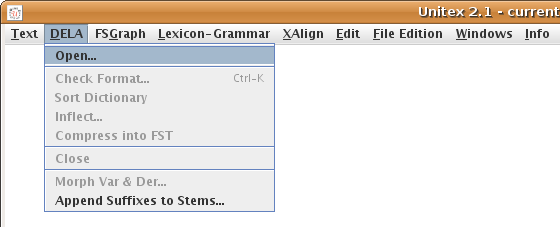
\includegraphics[width=13cm]{resources/img/fig3-1.png}
\caption{Menu "DELA"}
\end{center}
\end{figure}

\bigskip
\noindent
Si vous avez ouvert un dictionnaire, la fenêtrre affichée contient un champ qui vous permet
d'effectuer une recherche. Si le mot apparaît dans le dictionnaire, le bouton "Find" surligne la
première entrée correspondante. Si plusieurs entrées correspondent, vous pouvez les parcourir en
cliquant sur les deux boutons en forme de flèche.

\begin{figure}[!ht]
\begin{center}
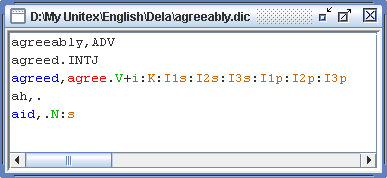
\includegraphics[width=7cm]{resources/img/fig3-2.png}
\caption{Recherche d'un mot dans un dictionnaire}
\end{center}
\end{figure}

\bigskip
\noindent
Vous pouvez aussi rechercher un mots dans plusieurs dictionnaires en cliquant sur le bouton "Lookup" du menu "DELA". Vous pouvez ensuite sélectionner les dictionnaires dans lesquels rechercher le mot que vous avez entré.

\begin{figure}[!ht]
\begin{center}
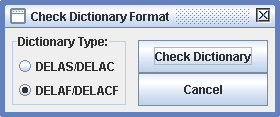
\includegraphics[width=7cm]{resources/img/fig3-3.png}
\caption{Recherche d'un mot dans plusieurs dictionnaires}
\end{center}
\end{figure}

\bigskip
\noindent

%%%%%%%%%%%%%%%%%%




\section{Vérification du format du dictionnaire}
\index{Dictionnaire!vérification} \index{Vérification du format d'un dictionnaire}
Lorsque les dictionnaires sont de taille importante, il devient fastidieux de les vérifier à
la main. Unitex contient le programme \verb+CheckDic+\index{Programmes externes!\verbc{CheckDic}}
\index{\verbc{CheckDic}} qui vérifie automatiquement les dictionnaires DELAF et DELAS.

\bigskip
\noindent Ce programme effectue une vérification de la syntaxe des entrées. Pour chaque entrée
mal formée, le programme affiche le numéro de ligne, le contenu de cette ligne et la nature
de l’erreur. Les résultats de l’analyse sont sauvés dans un fichier nommé
\verb+CHECK_DIC.TXT+\index{Fichier!\verbc{CHECK_DIC.TXT}} qui est affiché une fois la vérification
terminée. En plus des éventuels messages d’erreurs, ce fichier contient la liste de tous les
caractères utilisés dans les formes fléchies et canoniques, la liste des codes grammaticaux et
sémantiques,ainsi que la liste des codes flexionnels utilisés.
La liste des caractères permet de vérifier que les caractères présents dans le dictionnaire
sont cohérents avec ceux présents dans le fichier alphabet de la langue. Chaque caractère est
suivi par sa valeur en notation hexadécimale. Les listes de codes peuvent être utilisées pour
vérifier qu’il n’y a pas de faute de frappe dans les codes du dictionnaire.
\index{Fichier!alphabet}


\bigskip
\noindent Le programme \verb+CheckDic+ fonctionne avec des dictionnaires non comprimés, c’est-à-dire
sous forme de fichiers texte. La convention généralement appliquée est de donner l’extension
\verb+.dic+ \index{Fichier!\verbc{.dic}}. Pour vérifier le format d’un dictionnaire, il faut tout
d’abord l’ouvrir en cliquant sur "Open..." dans le menu "DELA".


\begin{figure}[!ht]
\begin{center}
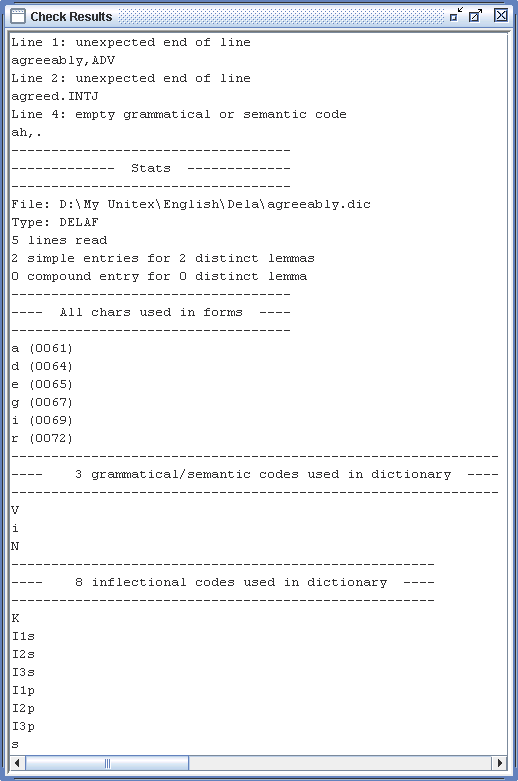
\includegraphics[width=10cm]{resources/img/fig3-4.png}
\caption{Exemple de dictionnaire\label{fig-dictionary-example}}
\end{center}
\end{figure}

\noindent Chargeons le dictionnaire de la figure~\ref{fig-dictionary-example}.
Pour lancer la vérification automatique, cliquez sur "Check Format..." dans le menu "DELA".
la fenêtre de la figure ~\ref{fig-dictionary-checking} apparaît alors.
Cette fenêtre vous permet de choisir le type du dictionnaire que vous voulez vérifier. Les
résultats de la vérification du dictionnaire de la figure~\ref{fig-dictionary-example},
 sont présentés sur la figure~\ref{fig-dictionary-checking-results}.

\bigskip
\noindent La première erreur est due au fait que le programme n’ait pas trouvé de point.
Le seconde, au fait qu’il n’ait pas trouvé de virgule marquant la fin de la forme fléchie.
La troisième erreur indique que le programme n’a trouvé aucun code grammatical ou sémantique.




\begin{figure}[!ht]
\begin{center}
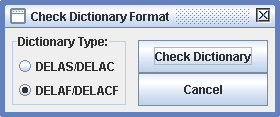
\includegraphics[width=7cm]{resources/img/fig3-5.png}
\caption{Vérification automatique d’un dictionnaire\label{fig-dictionary-checking}}
\end{center}
\end{figure}

\begin{figure}[!p]
\begin{center}
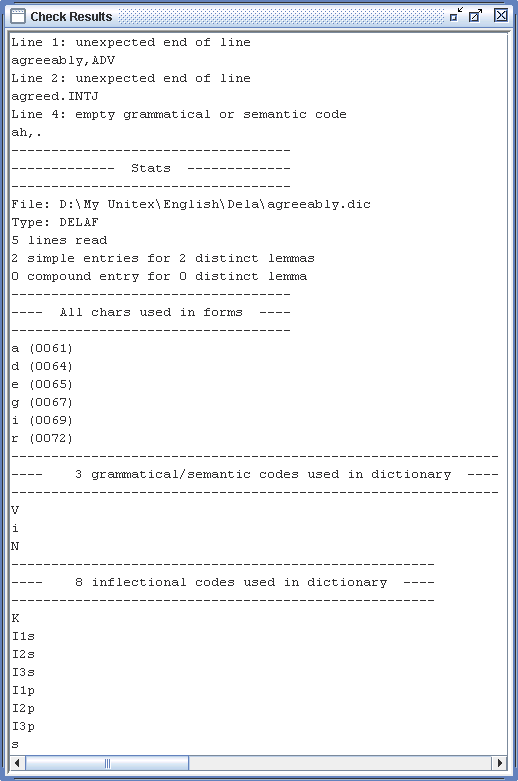
\includegraphics[height=19.4cm]{resources/img/fig3-6.png}
\caption{Résultats d’une vérification automatique\label{fig-dictionary-checking-results}}
\end{center}
\end{figure}


\section{Tri}
\index{Dictionnaire!tri}\index{Tri!d'un dictionnaire}

Unitex manipule les dictionnaires sans se soucier de l’ordre des entrées. Toutefois, pour
des raisons de présentation, il est souvent préférable de trier les dictionnaires. L’opération
de tri varie selon plusieurs critères, à commencer par la langue du texte à trier. Ainsi, le
tri d’un dictionnaire thaï s’effectue selon un ordre différent de l’ordre alphabétique, si bien
qu’Unitex utilise un mode de tri développé spécialement pour le thaï (voir chapitre
 \ref{chap-external-programs}).

\bigskip
\noindent Pour les langues européennes, le tri s’effectue généralement selon l’ordre
lexicographique, avec toutefois quelques variantes. En effet, certaines langues comme le français
considèrent certains caractères comme équivalents. Par exemple, la différence entre les caractères
\verb+e+ et \texttt{é} est ignorée lorsque l’on veut comparer les mots \verb+manger+ et
\texttt{mangés}, car les contextes \verb+r+ et \verb+s+ permettent de décider de l’ordre. La
distinction n’est faite que lorsque les contextes sont identiques, ce qui est le cas si l’on
compare \texttt{pêche} et \texttt{pèche}.

\bigskip \index{Alphabet!tri}
\noindent
Afin de prendre en compte ce phénomène, le programme de tri \verb+SortTxt+  
\index{\verbc{SortTxt}}\index{Programmes externes!\verbc{SortTxt}} utilise un fichier qui définit des
équivalences de caractères. \index{Équivalence de caractères}  Ce fichier s’appelle
\verb+Alphabet_sort.txt+ \index{Fichier!\verbc{Alphabet_sort.txt}} et se trouve dans le répertoire
de la langue courante de l’utilisateur. Voici les premières lignes du fichier utilisé par défaut
pour le français :


\bigskip
\begin{minipage}{\textwidth}
\noindent\texttt{AÀÂÄaàâä}

\noindent\texttt{Bb}

\noindent\texttt{CÇcç}

\noindent\texttt{Dd}

\noindent\texttt{EÉÈÊËeéèêë}
\end{minipage}

\bigskip
\noindent Les caractères présents sur une même ligne sont considérés comme équivalents quand
le contexte le permet. Lorsqu’il faut comparer deux caractères équivalents, on les compare
selon l’ordre dans lequel ils apparaissent de gauche à droite sur la ligne. On peut voir sur
l’extrait ci-dessus qu’on ne fait pas de différence entre minuscules et majuscules, et qu’on
ignore les accents ainsi que la cédille.


\bigskip
\noindent Pour trier un dictionnaire, ouvrez-le, puis cliquez sur "Sort Dictionary" dans le menu
"DELA". Par défaut, le programme cherche toujours à utiliser le fichier \verb+Alphabet_sort.txt+.
Si ce fichier est absent, le tri se fait selon l’indice des caractères dans le codage Unicode.
En modifiant ce fichier, vous pouvez définir vos propres préférences de tri.


\bigskip
\noindent Remarque : après l’application des dictionnaires sur un texte, les fichiers
\verb+dlf+, \verb+dlc+ et \verb+err+ sont automatiquement triés avec ce programme.
\index{Fichier!\verbc{dlf}} \index{Fichier!\verbc{dlc}}\index{Fichier!\verbc{err}}



\section{Flexion automatique}
\label{section-automatic-inflection}
\index{Flexion automatique}\index{Conjugaison}\index{Déclinaison}\index{Dictionnaire!flexion automatique}
\subsection{Flexion des mots simples}

Comme décrit dans la section~\ref{section-DELAS-format}, une ligne de DELAS se compose généralement
d’une forme canonique et d’une séquence de codes grammaticaux ou sémantiques :


\begin{verbatim}
aviatrix,N4+Hum
matrix,N4+Math
radix,N4
\end{verbatim}

\bigskip
\noindent Le premier code rencontré est interprété comme le nom de la grammaire à utiliser pour
fléchir la forme canonique. Il y a deux formes possibles :

\begin{itemize}
\item \verb+N4+: nom de la grammaire=\verb+N4.fst2+, codes grammaticaux=\verb+N+
	(le plus long préfixe uniquement composé de lettres)
  \item \verb+N(NC_XXX)+: nom de la grammaire=\verb+NC_XXX.fst2+, codes grammaticaux=\verb+N+
\end{itemize}

\bigskip
\noindent Ces grammaires de flexion\index{Grammaires!de flexion}\index{Graphe!de flexion}\index{Transducteur!de flexion}
seront automatiquement compilées si
besoin est. Dans l’exemple ci-dessus, toutes les entrées seront fléchies avec une grammaire nommée
\verb+N4+.

\bigskip
\noindent Pour lancer la flexion, cliquez sur "Inflect..." dans le menu "DELA". La fenêtre de la 
figure~\ref{fig-inflection-configuration} permet d’indiquer au programme de flexion le
répertoire dans lequel se trouvent les grammaires de flexion. Par défaut, le sous-répertoire
\verb+Inflection+ du répertoire de la langue courante est utilisé. On peut aussi spécifier quels
types de mots le dictionnaire est supposé contenir. Si une entrée non conforme est
rencontrée, un message d'erreur sera affiché.

\bigskip
\begin{figure}[!ht]
\begin{center}
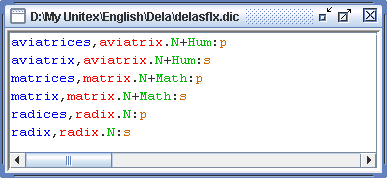
\includegraphics[width=8cm]{resources/img/fig3-7.png}
\caption{Configuration de la flexion automatique\label{fig-inflection-configuration}}
\end{center}
\end{figure}

\bigskip
\begin{figure}[!ht]
\begin{center}
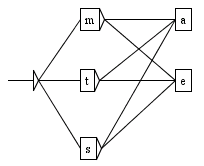
\includegraphics[width=4.5cm]{resources/img/fig3-8.png}
\caption{Grammaire de flexion
\texttt{N4}\label{fig-example-inflectional-grammar}}
\end{center}
\end{figure}

\bigskip
\noindent La figure~\ref{fig-example-inflectional-grammar} présente un exemple de grammaire de
flexion. Les chemins décrivent les suffixes à ajouter ou à retrancher pour obtenir la forme fléchie
à partir de la forme canonique, et les sorties (texte en gras sous les boîtes) donnent les codes
flexionnels à ajouter à l’entrée du dictionnaire.


\bigskip
\noindent Dans notre exemple, deux chemins sont possibles. Le premier ne modifie pas la forme
canonique et ajoute le code flexionnel \verb+:s+. Le second retranche une lettre grâce à l’opérateur 
\verb+L+, ajoute ensuite le suffixe \verb+ces+ et ajoute le code flexionnel \verb+:mp+.

Voici les opérateurs utilisables:

\begin{itemize}
\item \verb+L+ (left)\index{\verbc{L}}\index{Opérateur!\verbc{L}} enlève une lettre à l’entrée;
  	  
\item \verb+R+ (right)\index{\verbc{R}}\index{Opérateur!\verbc{R}}
             rétablit une lettre de l’entrée. En français, beaucoup de verbes du premier
  	  groupe se conjuguent au présent à la troisième personne du singulier en retirant le
  	  \verb+r+ de l’infinitif et en changeant la 4$\ieme$ lettre en partant de la fin en
  	  \texttt{è}: \verb+peler+ $\rightarrow$ \texttt{pèle},
  	  \verb+acheter+ $\rightarrow$ \texttt{achète}, \texttt{gérer}
  	  $\rightarrow$ \texttt{gère}, etc. Plutôt que d’écrire un suffixe de flexion
  	  pour chaque verbe (\texttt{LLLLèle}, \texttt{LLLLète} and
  	  \texttt{LLLLère}), on peut utiliser l’opérateur \verb+R+ pour n’en écrire qu’un seul :
  	  \texttt{LLLLèRR}.
  	  
\item \verb+C+ (copy)\index{\verbc{C}}\index{Opérateur!\verbc{C}}
             duplique une lettre de l’entrée, en décalant tout ce qui se trouve à sa droite.
  	  
Supposons par exemple que l’on souhaite générer automatiquement des adjectifs en
\verb+able+ à partir de noms. Dans des cas comme \verb+regrettable+ ou \verb+réquisitionnable+,
  on observe un doublement de la consonne finale du nom. Pour éviter d’écrire un
graphe de flexion pour chaque consonne finale possible, on peut utiliser l’opérateur
\verb+C+ afin de dupliquer la consonne finale, quelle qu’elle soit;
  
  \item \verb+D+ (delete)\index{\verbc{D}}\index{Opérateur!\verbc{D}}
             supprime une lettre de l’entrée, en décalant tout ce qui se trouve à sa  droite.
Si l’on souhaite par exemple fléchir le mot roumain \verb+european+ en \verb+europeni+, on utilisera
la séquence \verb+LDRi+. Le \verb+L+ positionnera le curseur sur la lettre \verb+a+, \verb+D+ va
supprimer le \verb+a+, en décalant le \verb+n+ sur la gauche, puis \verb+Ri+ va rétablir le \verb+n+
et ajouter un \verb+i+.

\item \verb+U+ (unaccent)\index{\verbc{U}}\index{Opérateur!\verbc{U}}
          enlève l'accent du caractère courant s'il en comporte un.
	Par exemple la séquence \verb+LLUx+ appliquée au mot
	\texttt{mangés} produit la forme fléchie \verb+mangex+, puisque \verb+U+
	à transformé le \texttt{é} en \verb+e+.

\item \verb+P+ (uppercase)\index{\verbc{P}}\index{Opérateur!\verbc{P}}
          met en majuscule la première lettre de la pile. Par exemple, la séquence
	\verb$Px$ transforme \verb$foo$ en \verb$Foox$.
  
\item \verb+W+ (lowercase)\index{\verbc{W}}\index{Opérateur!\verbc{W}}
          met en minuscule la première lettre de la pile.

\item \verb+<R=?>+ \index{\verbc{<R=?>}}\index{Opérateur!\verbc{<R=?>}}
          remplace la première lettre de la pile par la lettre \verb+?+.

\item \verb+<I=?>+ \index{\verbc{<I=?>}}\index{Opérateur!\verbc{<I=?>}}
          insère la lettre \verb+?+ avant la première lettre de la pile.

\item \verb+<X=n>+ \index{\verbc{<X=n>}}\index{Opérateur!\verbc{<X=n>}}
          supprime les $n$ premières lettres de la pile.
\end{itemize}

\noindent Il y a également deux opérateurs spéciaux pour le  Coréen:
\begin{itemize}\index{Jamo}\index{Hangul}
\item \verb+J+ \index{\verbc{J}}\index{Opérateur!\verbc{J}}
supprime une lettre Jamo. Si le caractère est un Hangul, ce caractère est d'abord
remplacé par sa séquence équivalente en alphabet Jamo, ensuite, la dernière lettre Jamo est
supprimée. Si le caractère n'est ni un Jamo, ni un Hangul, une erreur est produite.
\item \verb+.+ (latin dot)\index{\verbc{.}}\index{Opérateur!\verbc{.}}
           insère une limite de syllabe. Ceci a un effet de ford, si le haut de la
	pile contient des lettres Jamo, elles sont recombinées en Hangul.
\end{itemize}


\bigskip
\noindent Voici un exemple qui décrit la flexion de \verb+choose+ en \verb+chosen+
      grâce à la séquence d’opérateurs \verb+LLDRRn+ :
\begin{itemize}
  \item Étape 0: initialisation de la pile avec la forme canonique; on place le curseur après la
  	  dernière lettre:

\begin{center}
\begin{tabular}{|l|l|l|l|l|l|l|l}
\multicolumn{6}{l}{} & \multicolumn{2}{l}{$\downarrow$} \\
\hline
\verb+c+ & \verb+h+ & \verb+o+ & \verb+o+ & \verb+s+ & \verb+e+ & \verb+ + & \\
\hline
\end{tabular}
\end{center}

\bigskip
\item Étape 1: on décale le curseur vers la gauche:

\begin{center}
\texttt{\textbf{L}LDRRn}

\begin{tabular}{|l|l|l|l|l|l|l|l}
\multicolumn{5}{l}{} & \multicolumn{3}{l}{$\downarrow$} \\
\hline
\verb+c+ & \verb+h+ & \verb+o+ & \verb+o+ & \verb+s+ & \verb+e+ & \verb+ + & \\
\hline
\end{tabular}
\end{center}

\bigskip
\item Étape 2: on décale une seconde fois le curseur vers la gauche:

\begin{center}
\texttt{\textbf{LL}DRRn}

\begin{tabular}{|l|l|l|l|l|l|l|l}
\multicolumn{4}{l}{} & \multicolumn{4}{l}{$\downarrow$} \\
\hline
\verb+c+ & \verb+h+ & \verb+o+ & \verb+o+ & \verb+s+ & \verb+e+ & \verb+ + & \\
\hline
\end{tabular}
\end{center}

\bigskip \item Étape 3: on décale tout ce qui est à droite du curseur vers la gauche :

\begin{center}
\texttt{\textbf{LLD}RRn}

\begin{tabular}{|l|l|l|l|l|l|l|l}
\multicolumn{3}{l}{} & \multicolumn{5}{l}{$\downarrow$} \\
\hline
\verb+c+ & \verb+h+ & \verb+o+ & \verb+s+ & \verb+e+ & \verb+ + & \verb+ + & \\
\hline
\end{tabular}
\end{center}

\bigskip
\item Step 4: on décale le curseur vers la droite:

\begin{center}
\texttt{\textbf{LLDR}Rn}

\begin{tabular}{|l|l|l|l|l|l|l|l}
\multicolumn{4}{l}{} & \multicolumn{4}{l}{$\downarrow$} \\
\hline
\verb+c+ & \verb+h+ & \verb+o+ & \verb+s+ & \verb+e+ & \verb+ + & \verb+ + & \\
\hline
\end{tabular}
\end{center}

\bigskip
\item Step 5: on décale encore le curseur vers la droite:

\begin{center}
\texttt{\textbf{LLDRR}n}

\begin{tabular}{|l|l|l|l|l|l|l|l}
\multicolumn{5}{l}{} & \multicolumn{3}{l}{$\downarrow$} \\
\hline
\verb+c+ & \verb+h+ & \verb+o+ & \verb+s+ & \verb+e+ & \verb+ + & \verb+ + & \\
\hline
\end{tabular}
\end{center}

\bigskip
\item Step 6: on écrit un \verb+n+

\begin{center}
\texttt{\textbf{LLDRRn}}

\begin{tabular}{|l|l|l|l|l|l|l|l}
\multicolumn{6}{l}{} & \multicolumn{2}{l}{$\downarrow$} \\
\hline
\verb+c+ & \verb+h+ & \verb+o+ & \verb+s+ & \verb+e+ & \verb+n+ & \verb+ + & \\
\hline
\end{tabular}
\end{center}
\end{itemize}

\bigskip
\noindent Une fois la séquence d’opérateurs épuisée, on prend le contenu de la pile jusqu’avant le
curseur pour former la forme fléchie (ici \verb+chosen+).

\bigskip
\noindent Le programme de flexion \verb+Inflect+ explore tous les chemins de la grammaire de flexion
en engendrant toutes les formes fléchies possibles. Afin d’éviter de devoir remplacer les noms des
grammaires de flexion par de vrais codes grammaticaux dans le dictionnaire obtenu, le programme
remplace ces noms par leurs plus longs préfixes composés de lettres. Ainsi, \verb+N4+ est remplacé
par \verb+N+. En choisissant judicieusement les noms des grammaires de flexion, on peut donc
engendrer directement un dictionnaire prêt à l’emploi.

\bigskip
\noindent La figure \ref{fig-inflection-result} montre le dictionnaire obtenu après flexion du DELAS de notre exemple.

\bigskip
\begin{figure}[!ht]
\begin{center}
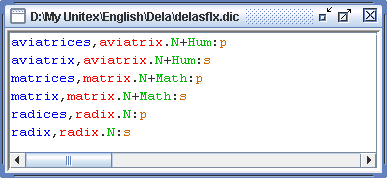
\includegraphics[width=9.5cm]{resources/img/fig3-9.png}
\caption{Résultat de la flexion automatique\label{fig-inflection-result}}
\end{center}
\end{figure}
\bigskip

\subsection{Opérateurs de flexion avancés}
\label{advanced-inflection-operators}
Dans certaines langues, le processus de flexion entraine une modification de la racine du mot.
Plusieurs opérateurs ont été développés pour faciliter ce type de traitement. Ils permettent de rechercher
et d'enlever un suffixe du mot \verb+W+ \`a fléchir. Cette opération peut
\^etre accompagnée de la mémorisation dans une variable (\$ ou \pounds) d'un facteur de ce suffixe.
Ces opérateurs peuvent prendre les formes suivantes~:

%\bigskip
\begin{itemize}
\item \verb+<X$Y>+~: On recherche à la fin du mot \verb+W+ le suffixe \verb+Y+.
	Puis, on recherche \`a partir de la position atteinte la {\bf plus proche} occurrence de \verb+X+
	qui précède strictement celle de \verb+Y+ . La variable \$ contient alors le {\bf plus court facteur}
	({\bf\$}hortest) de \verb+W+ strictement compris entre
	\verb+X+ et \verb+Y+ (\verb+W = U.X.$.Y+) \footnote{Le point représente ici l'opération de concaténation.}.
	L'opérateur \verb+<X$Y>+ retire \verb+X.$.Y+ de \verb+W+ et donne une valeur à \$. Une fois qu'il a été appliqué,
	la séquence qui reste dans la pile est \verb+U+, et la variable \$ peut être utilisée dans le reste du chemin.
\item \verb+<X£Y>+~: On recherche à la fin du mot \verb+W+ le suffixe \verb+Y+.
	Puis, on recherche \`a partir de la position atteinte l'occurrence de \verb+X+ la {\bf plus à gauche} qui
	précède strictement celle de \verb+Y+. La variable {\pounds} contient alors le {\bf plus long facteur}
	({\bf£}ongest) de \verb+W+ strictement compris entre \verb+X+ et \verb+Y+ (\verb+W = U.X.£.Y+).
\item \verb+<X>+~: Si aucune variable n'est présente, on recherche \verb+X+ comme suffixe de \verb+W+
	(\verb+W =U.X+).
\item \verb+<$Y>+: Si le facteur \verb+X+ est absent, le {\bf plus court facteur \verb+$+} est la première lettre
	qui précède strictement \verb+Y+ .
\item \verb+<£Y>+~: Si le facteur \verb+X+ est absent, le {\bf plus long facteur \verb+£+} est le préfixe de
	\verb+W+ tel que  \verb+W = £.Y+.
\end{itemize}

%\bigskip
\noindent
Pour illustrer l'utilisation des ces opérateurs, considérons le verbe {\it reprendre}~:

\bigskip
\begin{center}
\begin{tabular}{|l|l|l|l|}
\hline
Verbe     & Opérateur & Variable & Résultat\\
\hline
\hline
reprendre & <re> & & reprend\\
reprendre & <\$> & \$ = e & reprendr\\
reprendre & <{\pounds}> &{\pounds}= reprendre & $\varepsilon$ \\
reprendre & <re\$re> & \$ = nd & rep\\
reprendre & <re{\pounds}re> & {\pounds} = prend & \\
reprendre & <\$re> & \$ = d & repren\\
reprendre & <re\$> & \$ =  $\varepsilon$ & reprendre\\
reprendre & <{\pounds}re> & {\pounds} = reprend & $\varepsilon$\\
reprendre & <re{\pounds}> & {\pounds} = prendre & re\\
\hline
\end{tabular}
\end{center}

\bigskip
\noindent
Le programme MultiFlex permet d'utiliser dix variables de type \$ dont les noms sont \$, \$1..., \$9
et dix variables de type {\pounds} dont les noms sont {\pounds}, {\pounds}1..., {\pounds}9. De plus,
plusieurs variables de types différents peuvent \^etre utilisées au sein d'une m\^eme opération.
Ainsi l'opérateur <{\pounds}3re\$7re> appliqué au verbe {\it reprendre} donne {\pounds}3 = 
 rep et \$7 = \verb+nd+.

\bigskip
\noindent
Si l'on considère les verbes \verb+accélérer+, \verb+sécher+, la
deuxième personne du présent de l'indicatif peut \^etre générée par l'opération <é\$er>è\$es~:

\begin{center}
\begin{tabular}{lllllllll}
	\verb+accélérer+ & <é\$er> & $\rightarrow$ & accél & \$ = r & + & è\$es &  $\rightarrow$ & \verb+accélères+\\
	\verb+sécher+ & <é\$er> & $\rightarrow$ & s & \$ = ch & + & è\$es & $\rightarrow$ & \verb+sèches+\\
\end{tabular}
\end{center}

\noindent
On remarque que le facteur \verb+$+ conservé dans la forme fléchie est de longueur variable (\verb+r+, \verb+ch+). 
La flexion de \verb+accélérer+ et \verb+sécher+ ne peut se faire que par des opérateurs de pile
classiques \`a l'aide d'une opération commune. Deux opérations différentes (\verb+-4RèCes+, \verb+-5RèCes+) sont
nécessaires. Le graphe de la figure~\ref{fig-inflection-secher} permet de fléchir des verbes comme
\verb+accélérer+ et \verb+sécher+ au présent.

\begin{figure}[!ht]
\begin{center}
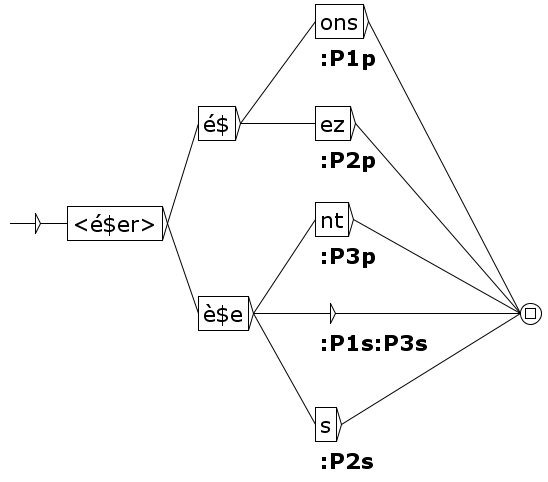
\includegraphics[width=7cm]{resources/img/fig3-Advanced_operators_with_Variables-V_secher.png}
\caption{Graphe de flexion pour des verbes comme {\it accélérer}, {\it sécher}
\label{fig-inflection-secher}}
\end{center}
\end{figure}

\newpage
\noindent
Voici les flexions obtenues pour les verbes \verb+accélérer+ et \verb+sécher+:

\begin{figure}[!ht]
\begin{center}
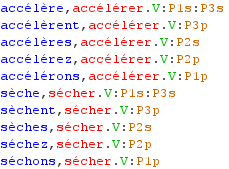
\includegraphics[width=5cm]{resources/img/fig3-flexion_secher.png}
\end{center}
\end{figure}

\bigskip
\noindent
Le redoublement de certaines lettres lors de la flexion peut s'effectuer avec l'opérateur \$.
Par exemple l'adject {\it tranquil} en anglais possède deux formes au comparatif et deux au
superlatf. Le graphe de la figure ~\ref{fig-inflection-tranquil} permet de les produire.

\bigskip
\begin{figure}[!ht]
\begin{center}
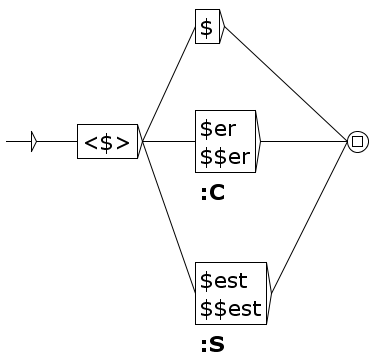
\includegraphics[width=5.5cm]{resources/img/fig3-Advanced_operators_with_Variables-A_tranquil.png}
\caption{Graphe de flexion pour des adjectifs anglais comme {\it tranquil}
\label{fig-inflection-tranquil}}
\end{center}
\end{figure}

\noindent Voici les flexions obtenues pour l'adjectif anglais \verb+tranquil+:

\bigskip
\begin{figure}[!ht]
\begin{center}
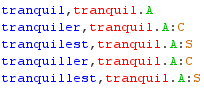
\includegraphics[width=5cm]{resources/img/fig3-flexion_tranquil.png}
\end{center}
\end{figure}

\noindent Dans certaines langues, certaines formes fléchies comporte un préfixe qui s'ajoute devant la racine.
C'est le cas lors de la formation du participe passé en allemand. L'utilisation conjointe des
opérateurs \verb+£+ et \verb+$+ permet de fléchir le verbe allemand \verb+sprechen+ (parler)
au présent et participe passé comme le montre le graphe de la figure~\ref{fig-inflection-sprechen}.

\newpage
\begin{figure}[!htbp]
\begin{center}
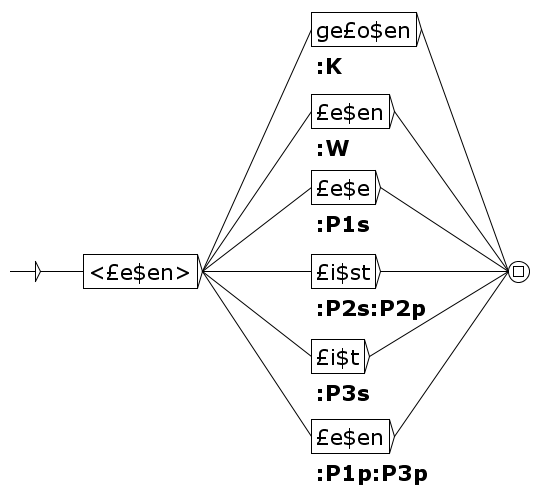
\includegraphics[width=5cm]{resources/img/fig3-Advanced_operators_with_Variables-V_sprechen.png}
\caption{Graphe de flexion pour des verbes comme {\it sprechen}
\label{fig-inflection-sprechen}}
\end{center}
\end{figure}

\noindent Voici les flexions obtenues pour le verbe allemand \verb+sprechen+:

\bigskip
\begin{figure}[!ht]
\begin{center}
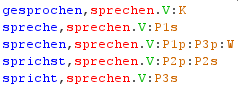
\includegraphics[width=5cm]{resources/img/fig3-flexion_sprechen.png}
\end{center}
\end{figure}

\noindent Si l'on veut fléchir le verbe à particule aussprechen on peut utiliser deux variables de type \$.
Le figure ~\ref{fig-inflection-aussprechen} montre un graphe qui comport les variables \verb+$1+ et \verb+$2+.

\bigskip
\begin{figure}[!ht]
\begin{center}
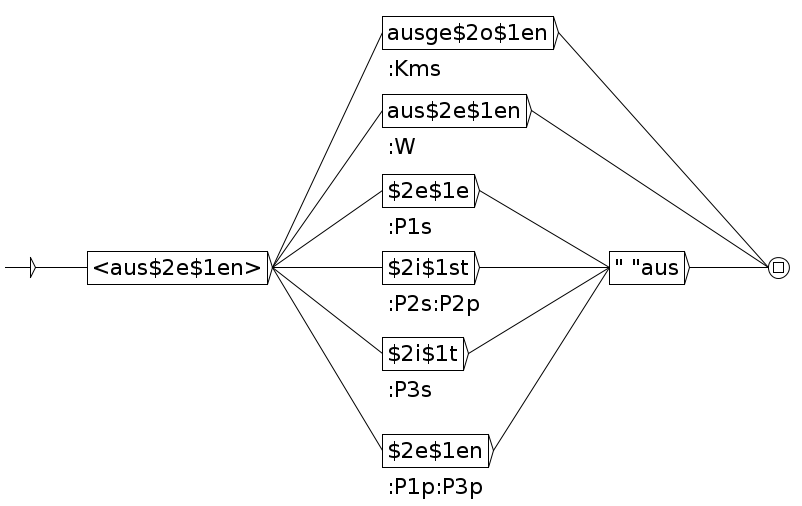
\includegraphics[width=10.5cm]{resources/img/fig3-Advanced_operators_with_Variables-V_aussprechen.png}
\caption{Graphe de flexion pour des verbes comme {\it aussprechen}
\label{fig-inflection-aussprechen}}
\end{center}
\end{figure}

\noindent Voici les flexions obtenues pour le verbe allemand \verb+aussprechen+:
\bigskip
\begin{figure}[!ht]
\begin{center}
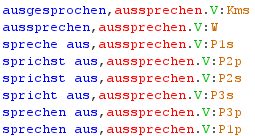
\includegraphics[width=5cm]{resources/img/fig3-flexion_aussprechen2.png}
\end{center}
\end{figure}

\bigskip
\noindent \textbf{Codes sémantiques}
\noindent Dans certaines langues, il existe des caractéristiques flexionnelles qui correspondent
en fait à des caractéristiques sémantiques comme par exemple les marqueurs de la forme passive.
Ces codes peuvent ne pas apparaître comme des codes flexionnels, mais plutôt comme des codes
sémantiques. Pour produire des codes sémantiques, il faut insérer un signe plus au début de la
sortie d'une boîte. Cette boîte doit seulement contenir le code sémantique précédé d'un plus, comme
le montre la figure~\ref{fig-inflection-sem}.

\bigskip
\begin{figure}[!ht]
\begin{center}
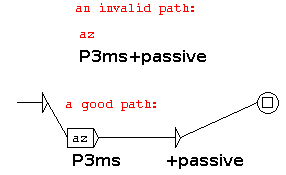
\includegraphics[width=6cm]{resources/img/fig3-9sem.png}
\caption{Une grammaire de flexion avec un code sémantique\label{fig-inflection-sem}}
\end{center}
\end{figure}


\subsection{Flexion des mots composés}
Voir chapitre \ref{chap-multiflex}.


\subsection{Flexion des langues sémitiques}
\label{subsection-semitic-inflection}
\index{Langues sémitiques}
Les langues  sémitiques comme l'arabe ou l'hébreu se fléchissent d'une manière qui n'est pas facilement représentable
avec les opérateurs de flexion décrits ci-dessus. Leur morphologie obéit à une logique différente~:
les mots se fléchissent selon un \textit{squelette consonantique}\index{Squelette consonantique}.
Le processus de flexion combine ce squelette avec des voyelles.
Des opérateurs spécifiques ont été implémentés pour les langues sémitiques, et certains pourraient être utiles
aussi pour des langues en dehors de la famille sémitique, comme le tagalog.

\bigskip
\noindent Tout d'abord, voyons un cas où on ne code que les consonnes dans le champ lemme de l'entrée DELAS~:

\bigskip
\noindent \verb+ktb,$V31-123+

\bigskip
\noindent Le signe \verb+$+ avant le code grammatical indique que la grammaire de flexion est en mode sémitique, et
la forme \verb+ktb+ qui figure dans le champ lemme est le squelette consonantique. La figure \ref{semitic-grammar}
montre une grammaire jouet \verb+V31-123.grf+ qui illustre le fonctionnement du mode sémitique. Les grammaires
de flexion utilisent la translittération Buckwalter++ de l'écriture arabe (cf.~section~\ref{transliteration-Arabic}).

\bigskip
\begin{figure}[!ht]
\begin{center}
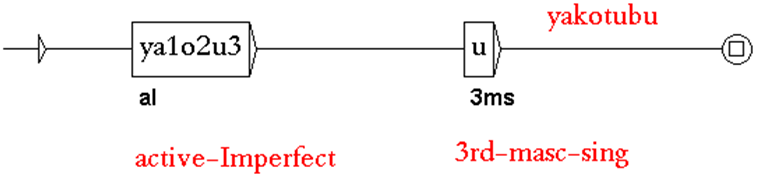
\includegraphics[width=10cm]{resources/img/fig3-15.png}
\caption{Une grammaire de flexion jouet en mode sémitique\label{semitic-grammar}}
\end{center}
\end{figure}

\noindent Le mode sémitique obéit aux règles suivantes:
\begin{enumerate}
\item Tous les opérateurs de flexion standard peuvent être utilisés (\verb+L+, \verb+R+, etc.).
\item Un chiffre représente une lettre du champ lemme (\verb+1+ pour la première,
\verb+2+ pour la seconde, etc). Dans notre exemple, \verb+1+, \verb+2+ et \verb+3+ représentent
respectivement \verb+k+, \verb+t+ et \verb+b+. Si on veut désigner une lettre après la neuvième,
on doit protéger son numéro avec des chevrons~: \verb+<10>+.
\end{enumerate}  

\noindent Le DELAF produit par cette grammaire est:\\ 
  
\verb+yakotubu,ktb.V:aI3ms+

\bigskip
\noindent Si on ne code que les consonnes dans le champ lemme et que deux entrées ont les mêmes
consonnes mais diffèrent par leurs voyelles, on doit coder les voyelles dans les grammaires de flexion~:\\ 

\verb+Hsb,$V3au	// compter, Hasaba, yaHosubu+

\verb+Hsb,$V3ii	// penser, Hasiba, yaHosibu+

\begin{figure}[!ht]
\begin{center}
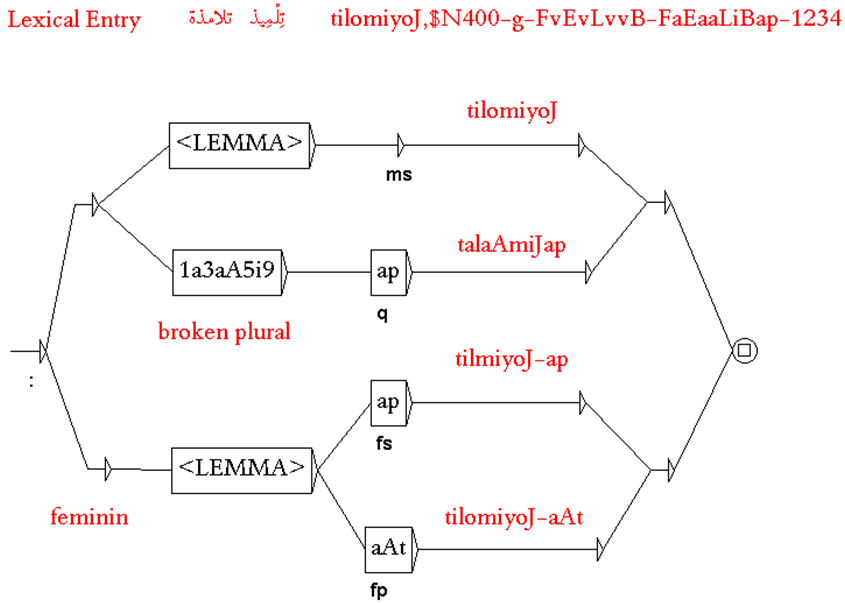
\includegraphics[width=10cm]{resources/img/fig3-LEMMA-operator.png}
\caption{Une grammaire de flexion en mode sémitique avec l'opérateur <LEMMA>\label{LEMMA-operator}}
\end{center}
\end{figure}

\bigskip
\noindent Pour copier tout le champ lemme, on peut utiliser l'opérateur <LEMMA>.
Une boite contenant cet opérateur récupère tout le champ lemme mais ne dépend pas du nombre de lettres.
Cet opérateur est utile pour les noms et adjectifs arabes pour lesquels les formes du masculin sont obtenues en
insérant des voyelles dans le squelette consonantique, alors que celles du féminin le sont en ajoutant des
suffixes (figure~\ref{LEMMA-operator}). Dans cet exemple, on a codé à la fois les consonnes et les voyelles
dans le champ lemme.

\bigskip
\noindent L'opérateur <n.LEMMA>  copie le lemme depuis la $n$ième position jusqu'à la fin.
Par exemple, dans certains noms arabes, la voyelle brève de la première syllabe alterne~:
\verb+a/u+, \verb+a/i+ ou \verb+u/i+, comme dans \verb+nufaAyap+/\verb+nifaAyap+ ''ordures''.
La grammaire de flexion de la fig.~\ref{n.LEMMA-operator} produit à la fois les variantes en \verb+u+ et en  \verb+i+
comme formes fléchies de \verb+nufaAyap+.

\begin{figure}[!ht]
\begin{center}
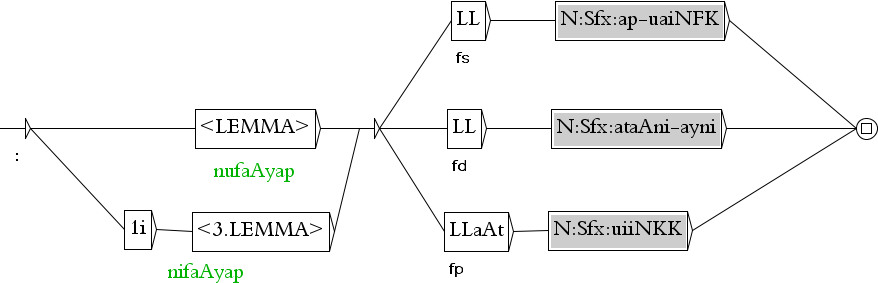
\includegraphics[width=14cm]{resources/img/N0_i_0ap-f-At.png}
\caption{Une grammaire de flexion en mode sémitique avec l'opérateur <n.LEMMA>\label{n.LEMMA-operator}}
\end{center}
\end{figure}

\bigskip
\noindent En tagalog, une langue austronésienne parlée aux Philippines et qui utilise communément des infixes
et des redoublements pour la flexion, <LEMMA> et <n.LEMMA> peuvent être utiles pour produire des temps verbaux.
La grammaire de flexion jouet de la fig.~\ref{tagalog} produit le parfait \verb+kumain+, le futur \verb+kakain+
et l'imparfait \verb+kumakain+ du verbe \verb+kain+ ''manger''.

\begin{figure}[!ht]
\begin{center}
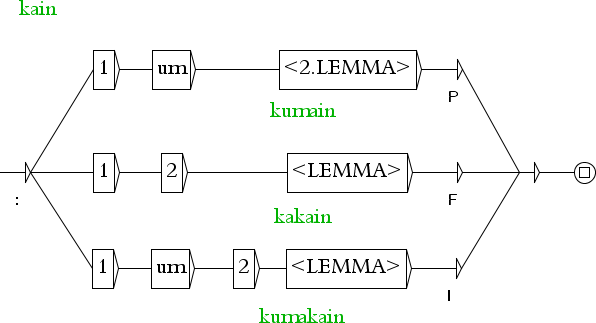
\includegraphics[width=12cm]{resources/img/V1um.png}
\caption{Une grammaire de flexion jouet pour le tagalog en mode sémitique\label{tagalog}}
\end{center}
\end{figure}

\section{Translittération des dictionnaires d'arabe}
\index{Translittération!arabe}\index{Dictionnaires!translittération}

Quand les linguistes arabes analysent des dictionnaires pour y détecter des erreurs,
la lecture dans l'écriture arabe est simple et efficace. Cependant, quand ils
créent des grammaires de flexion (section~\ref{section-automatic-inflection}), des éléments
de mots arabes apparaissent dans la même boite que des informations morpho-syntaxiques
codées dans l'alphabet latin, et dans ce contexte, les allers-retours entre l'écriture arabe,
qui se lit de droite à gauche, et l'alphabet latin, qui se lit de gauche à droite, ne sont pas
pratiques. Avec Unitex, on peut coder des grammaires de flexion entièrement dans l'alphabet
latin, en utilisant la translittération Buckwalter++,\index{Buckwalter++} une correspondance
biunivoque entre un codage Unicode de l'écriture arabe et des lettres de l'alphabet latin
(cf.~\cite{neme2011}, section~3.2, pp.~4--6). La translittération Buckwalter++ est définie
par la table des figures~\ref{buckwalter1} et \ref{buckwalter2}.
Unitex offre une fonctionnalité de translittération de dictionnaires DELAS et DELAF de l'arabe
vers le code Buckwalter++ et inversement (fig.~\ref{Arabic-transliteration}). Cette fonctionnalité
est accessible par le menu DELA.

\begin{figure}[!p]
\begin{center}
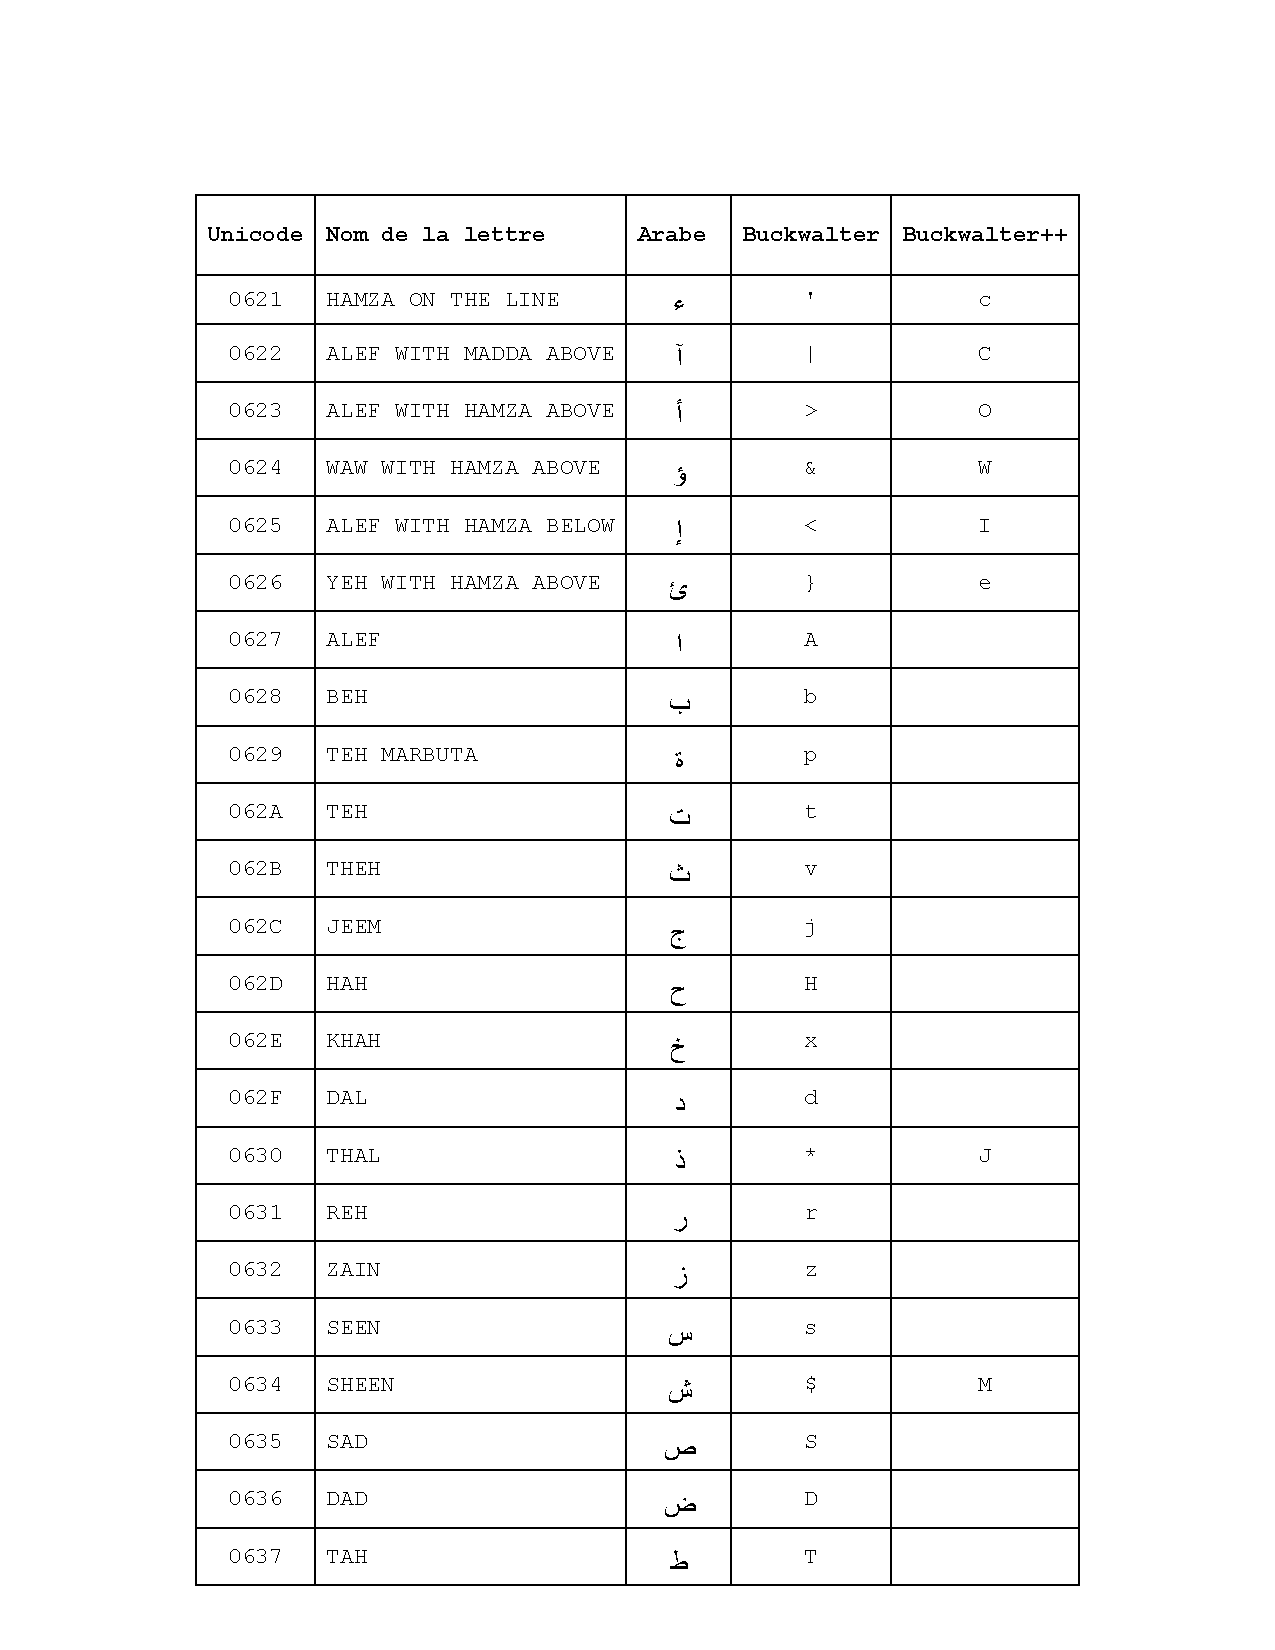
\includegraphics[height=23.5cm]{resources/img/buckwalter1-fr.pdf}
\caption{Table de translittération Buckwalter++, première moitié\label{buckwalter1}}
\end{center}
\end{figure}

\begin{figure}[!p]
\begin{center}
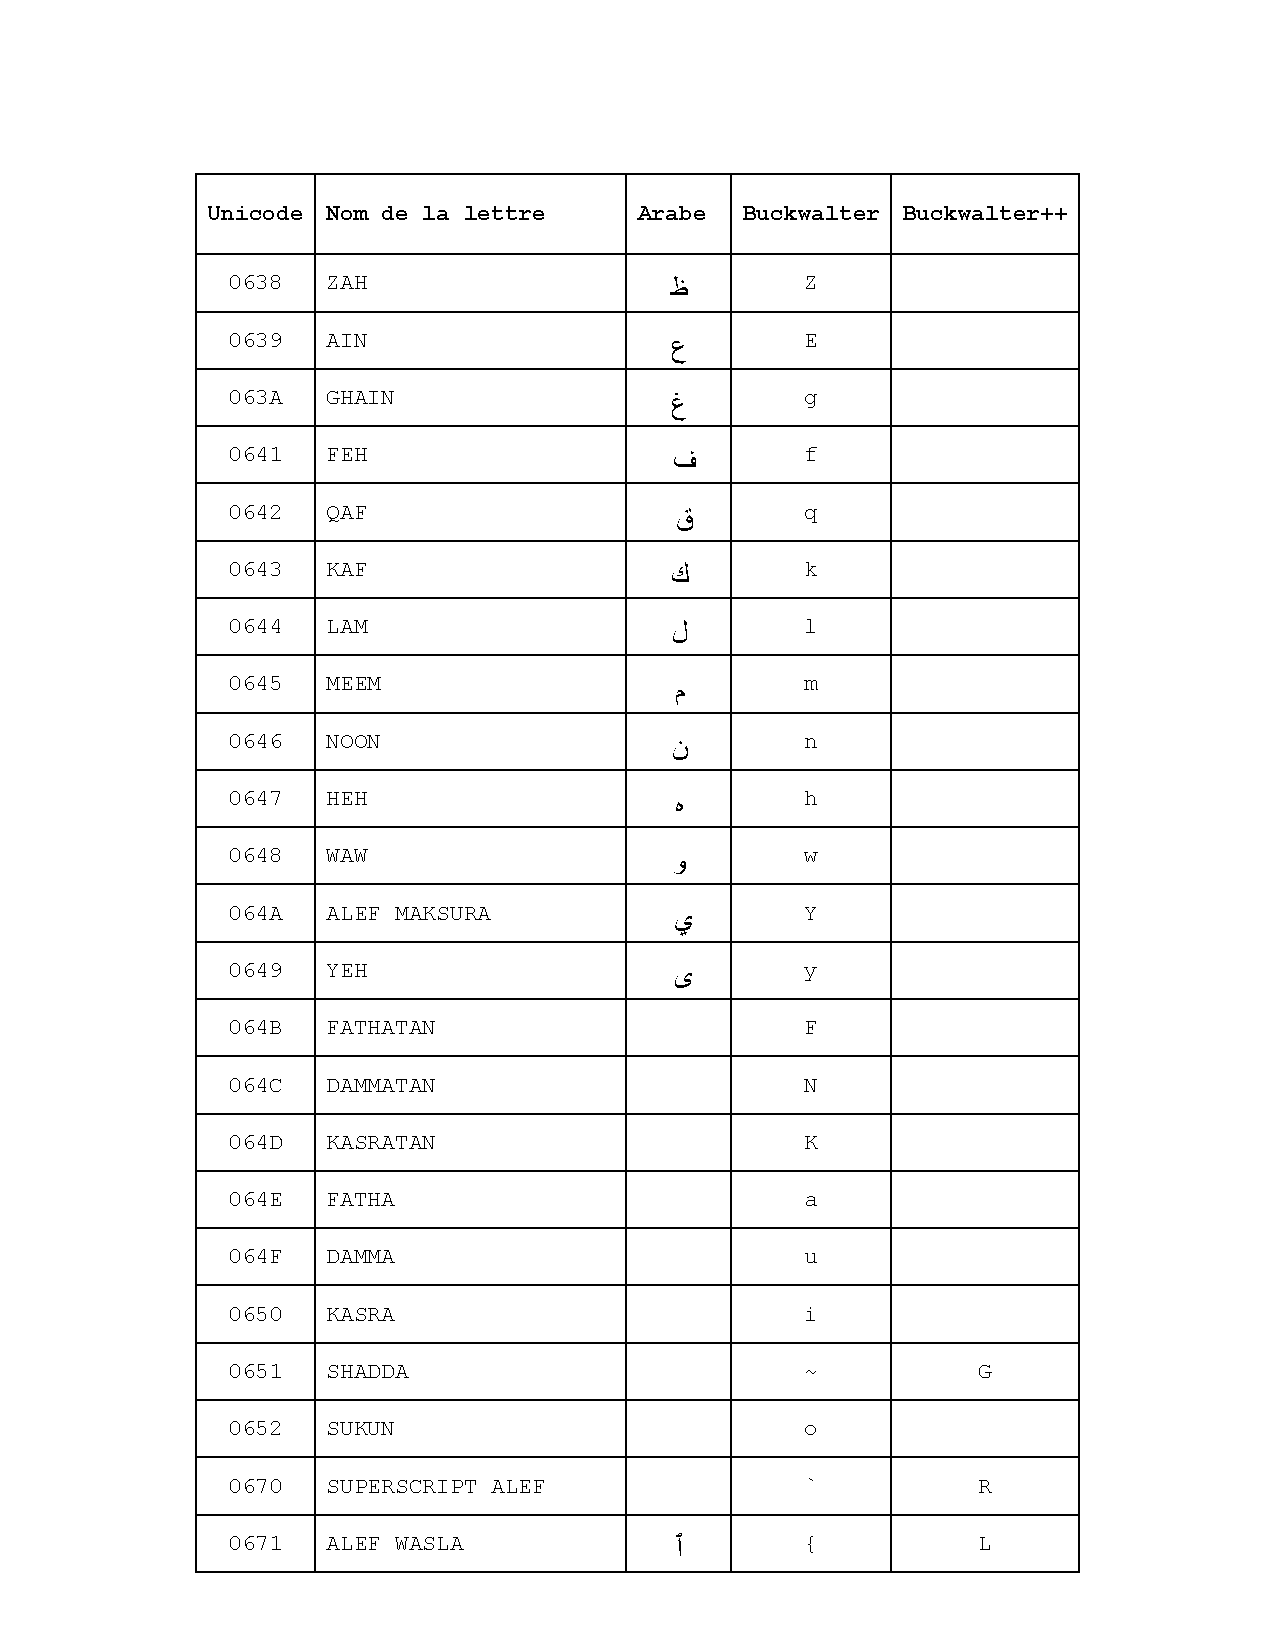
\includegraphics[height=23.5cm]{resources/img/buckwalter2-fr.pdf}
\caption{Table de translittération Buckwalter++, deuxième moitié\label{buckwalter2}}
\end{center}
\end{figure}

\begin{figure}[!ht]
\begin{center}
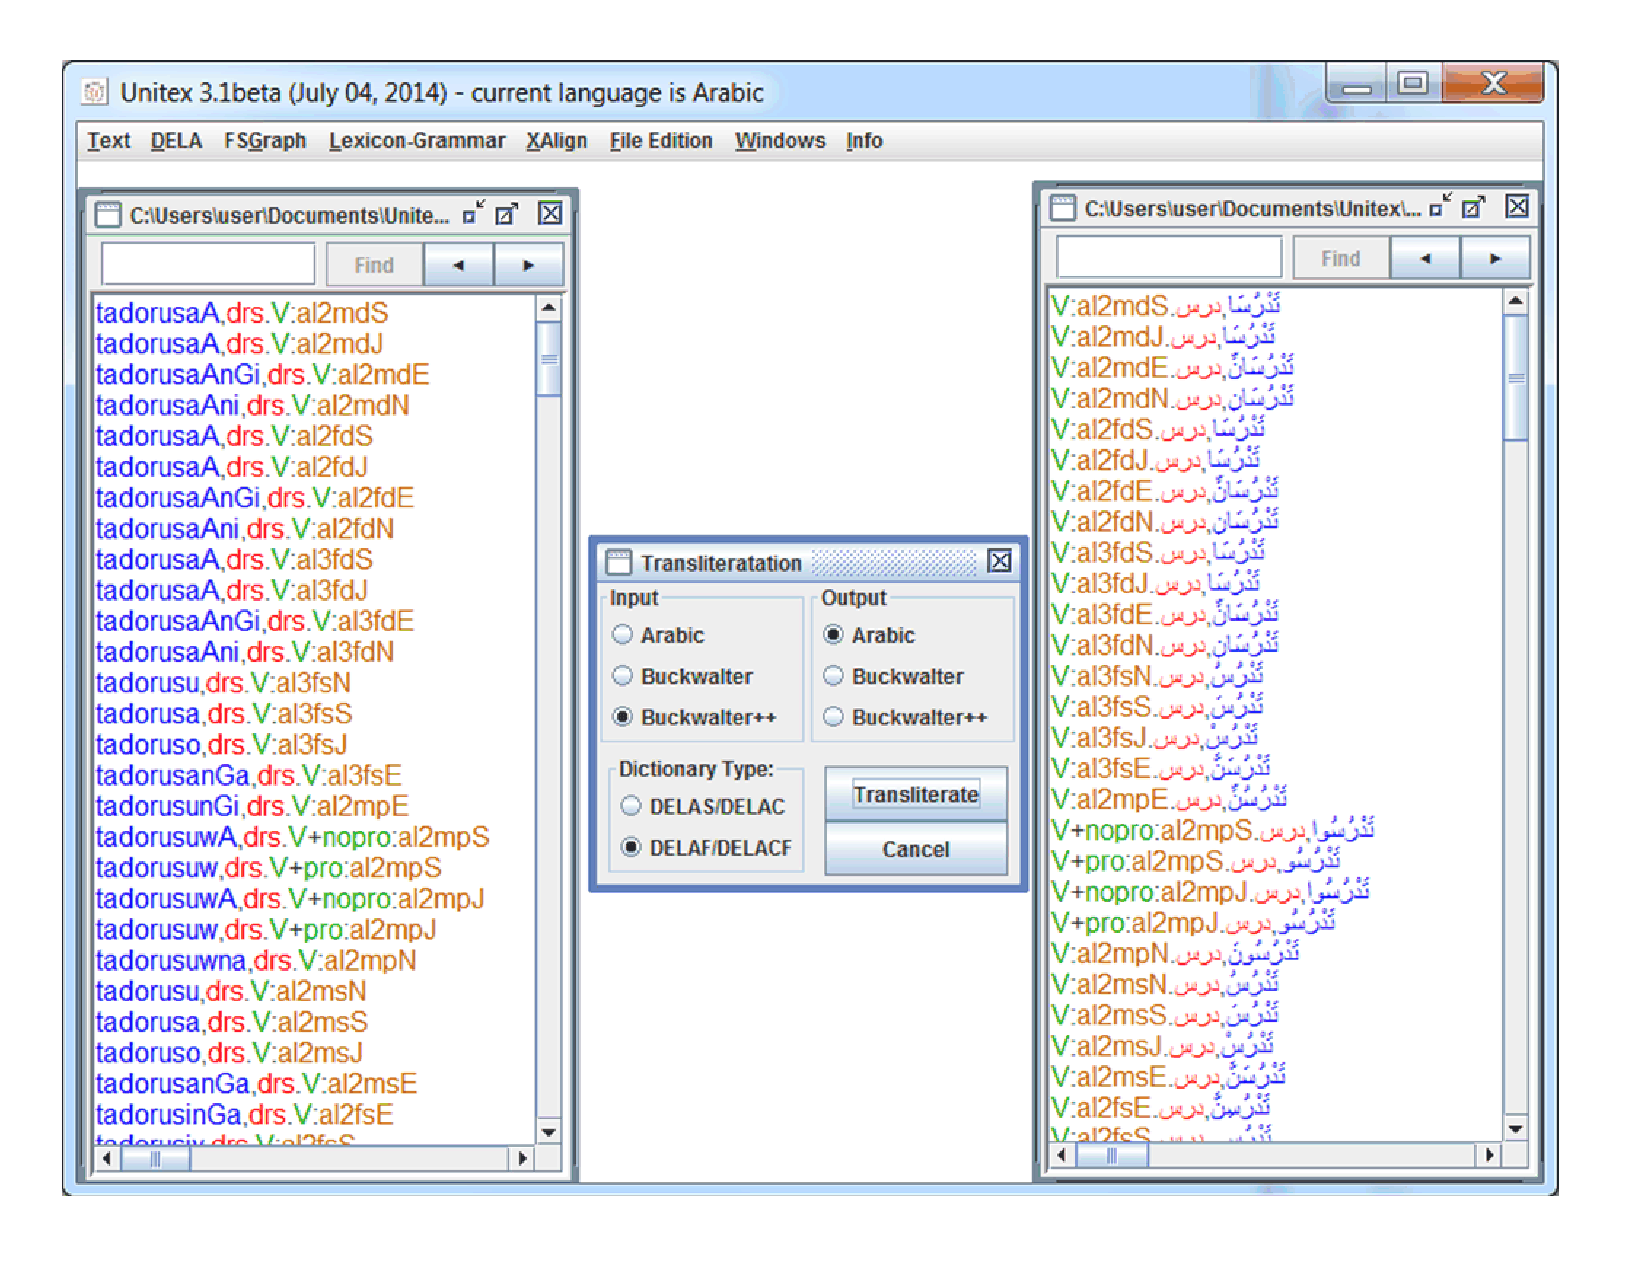
\includegraphics[width=15cm]{resources/img/Arabic-transliteration.pdf}
\caption{Translittération d'un dictionnaire DELAF
depuis le code Buckwalter++ (à gauche) vers l'écriture arabe (à droite)\label{Arabic-transliteration}}
\end{center}
\end{figure}


\section{Compression}
\index{Dictionnaire!compression}

Unitex applique aux textes des dictionnaires comprimés. La compression permet de réduire
la taille des dictionnaires et d’en accélérer la consultation. Cette opération s’effectue
avec le programme \verb+Compress+. \index{\verbc{Compress}}\index{Programmes externes!\verbc{Compress}}
Celui-ci prend en entrée un dictionnaire sous forme de fichier texte (par exemple
	\verb+mon_dico.dic+) et produit deux fichiers:\index{Fichier!\verbc{.dic}}

\begin{itemize}
  \item \verb+mon_dico.bin+ contient l’automate minimal des formes fléchies du dictionnaire;
  	  \index{Fichier!\verbc{.bin}}
  \item \verb+mon_dico.inf+ \index{Fichier!\verbc{.inf}}contient des codes qui permettent de
  	  reconstruire le dictionnaire d’origine à partir
  	  des formes fléchies contenues dans \verb+mon_dico.bin+.
\end{itemize}

\index{Automate!minimal}
\noindent L’automate minimal contenu dans \verb+mon_dico.bin+ est une représentation des formes
fléchies où tous les préfixes et suffixes
communs sont factorisés. Par exemple, l’automate minimal des mots \verb+me+, \verb+te+, \verb+se+,
\verb+ma+, \verb+ta+ et \verb+sa+
peut être représenté par le graphe de la figure~\ref{fig-example-minimal-automaton}.
\bigskip \begin{figure}[!ht]
\begin{center}
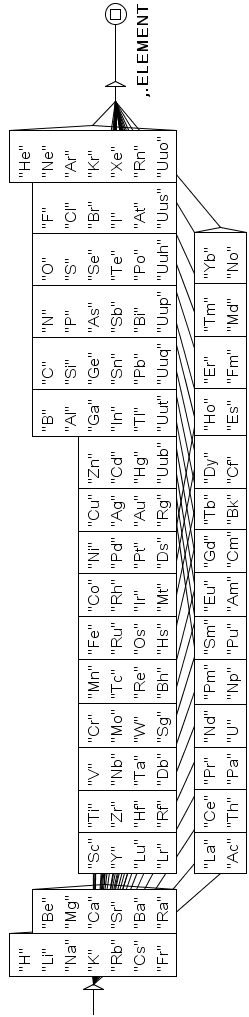
\includegraphics[width=5cm]{resources/img/fig3-10.png}
\caption{Représentation d’un exemple d’automate minimal\label{fig-example-minimal-automaton}}
\end{center}
\end{figure}

\noindent    Pour comprimer un dictionnaire, ouvrez-le puis cliquez sur "Compress into FST" dans le
menu "DELA". La compression est indépendante de la langue et du contenu du dictionnaire.
Les messages produits par le programme sont affichés dans une fenêtre qui ne se ferme pas
automatiquement. Vous pouvez ainsi voir la taille du fichier
\verb+.bin+, obtenu, le nombre de lignes lues ainsi que le nombre de codes flexionnels produits. La
figure ~\ref{fig-compression-result}
montre le résultat de la compression d’un dictionnaire de mots simples.

\bigskip
\begin{figure}[!ht]
\begin{center}
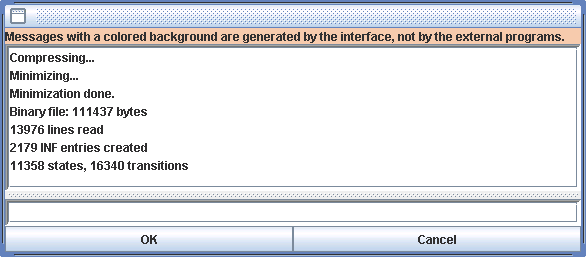
\includegraphics[width=14cm]{resources/img/fig3-11.png}
\caption{Résultat d’une compression\label{fig-compression-result}}
\end{center}
\end{figure}

\bigskip
\noindent À titre indicatif, les taux de compression généralement observés sont d’environ 95\% pour
les dictionnaires de mots simples et 50\% pour ceux de mots composés.


\bigskip
\noindent Quand le mode sémitique (\ref{subsection-semitic-inflection}) a beaucoup été utilisé lors de la flexion
d'un dictionnaire, une variante spécifique de l'algorithme de compression peut réduire la taille des fichiers
\verb+.bin+ et \verb+.inf+. Pour l'invoquer, soit on déclare la langue comme étant sémitique dans les préférences
globales, en cochant l'option ''Semitic language'' dans ''Preferences > Language and Presentation'', soit on
lance le programme Compress en ligne de commande avec l'option \verb+--semitic+.


\section{Application de dictionnaires}
\label{section-applying-dictionaries}
\index{Dictionnaire!application}

\bigskip
\noindent Unitex peut manipuler soit des dictionnaires compressés (\verb+.bin+) soit des graphes-dictionnaires (\verb+.fst2+). Ces dictionnaires peuvent être appliqués soit lors du prétraitement,
soit explicitement en cliquant sur "Apply Lexical Resources..." dans le menu "Text". Nous allons
maintenant détailler les règles de l’application des dictionnaires. Le cas des graphes-dictionnaires
sera abordé dans la section ~\ref{section-dictionary-graphs}.

\subsection{Priorités}
\label{section-dictionary-priorities}
\index{Dictionnaire!priorité}\index{Priorité!entre dictionnaires}
La règle de priorité est la suivante : si un mot du texte a été trouvé dans un dictionnaire,
ce mot ne sera plus pris en compte lors de l’application de dictionnaires ayant une priorité
inférieure.


\bigskip
\noindent Cela permet d’éliminer certaines ambiguïtés lors de l’application des dictionnaires.
Par exemple, le mot \textit{par} a une interprétation nominale dans le domaine du golf. Si l’on ne
veut pas envisager cet emploi, il suffit de créer un dictionnnaire filtre ne contenant que l’entrée 
\verb$par,.PREP$ et de le sauver en lui donnant la priorité la plus haute. De cette manière, même
si le dictionnaire des mots simples contient l’autre entrée, celle-ci sera ignorée grâce au jeu
des priorités.

\index{Dictionnaire!filtre}

\bigskip
\noindent Il y a trois niveaux de priorités. Les dictionnaires dont les noms sans extension se
terminent par \verb+-+\index{\verbc{-}}\index{\verbc{+}} ont la priorité la plus grande ; ceux dont
le nom se termine par \verb-+- ont la priorité la plus faible ; les autres dictionnaires sont
appliqués avec une priorité moyenne. L’ordre d’application de plusieurs dictionnaires ayant la même
priorité est sans importance. En ligne de commande, l’instruction :


\bigskip
\noindent
\verb$Dico ex.snt alph.txt ctr+.bin cities-.bin rivers.bin regions-.bin$

\bigskip \noindent appliquerait donc les dictionnaires dans l’ordre suivant (\verb+ex.snt+ est le
texte auquel sont appliqués les dictionnaires, \verb+alph.txt+ est le fichier alphabet utilisé):

\begin{enumerate}
  \item \verb$cities-.bin$
  \item \verb$regions-.bin$
  \item \verb$rivers.bin$
  \item \verb$ctr+.bin$
\end{enumerate}

\subsection{Règles d’application des dictionnaires}
\label{section-transducer-application-rules}

Outre la règle de priorités, l’application des dictionnaires s’effectue en respectant les
majuscules et les espaces. La règle du respect des majucules est la suivante :

\index{Règles!majuscules et minuscules}

\begin{itemize}
  \item s’il y a une majuscule dans le dictionnaire, alors il doit y avoir une majuscule dans le
texte ;

  \item s’il y a une minuscule dans le dictionnaire, il peut y avoir soit une minuscule soit une
majuscule dans le texte.

\end{itemize}

\noindent Ainsi, l’entrée \verb$pierre,.N:fs$ reconnaîtra les mots \verb+pierre+,
\verb+Pierre+ et \verb+PIERRE+, alors que

\noindent \verb$Pierre,.N+Prénom$ ne reconnaîtra que \verb+Pierre+ et \verb+PIERRE+. Les lettres
minuscules et majuscules sont définies par le fichier alphabet passé en paramètre au programme
\verb+Dico+\index{\verbc{Dico}}\index{Programmes externes!\verbc{Dico}}
\index{Fichier!\verbc{Alphabet.txt}}\index{Fichier!alphabet}\index{Alphabet}.\index{Règles!espace}

\bigskip
\noindent Le respect des espacements est une règle très simple : pour qu’une séquence du texte
soit reconnue par une entrée de dictionnaire, elle doit avoir exactement les mêmes espaces.
Par exemple, si le dictionnaire contient \verb+aujourd'hui,.ADV+, la séquence \verb+Aujourd' hui+
ne sera pas reconnue à cause de l’espace qui suit l’apostrophe.


\subsection{Graphes-dictionnaires}
\label{section-dictionary-graphs}\index{Graphe!dictionnaire}\index{Graphe-dictionnaire}
Le programme \verb+Dico+\index{\verbc{Dico}}\index{Programmes externes!\verbc{Dico}} est également capable
d’appliquer des graphes-dictionnaires. Il s’agit de graphes qui respectent,
par défaut\footnote{Les graphes-dictionnaires morphologiques sont une exception
(section~\ref{section-morphological-dictionary-graphs}) .}, la règle suivante :
si on les applique avec le programme \verb+Locate+\index{\verbc{Locate}}\index{Programmes externes!\verbc{Locate}} en mode MERGE,\index{MERGE} ils doivent produire des séquences
correspondant à des lignes de DELAF.\index{DELAF}\index{Dictionnaire!DELAF}
Quand on les applique à un texte, ils attachent les étiquettes lexicales DELAF à ces séquences.


\begin{figure}[!p]
\begin{center}
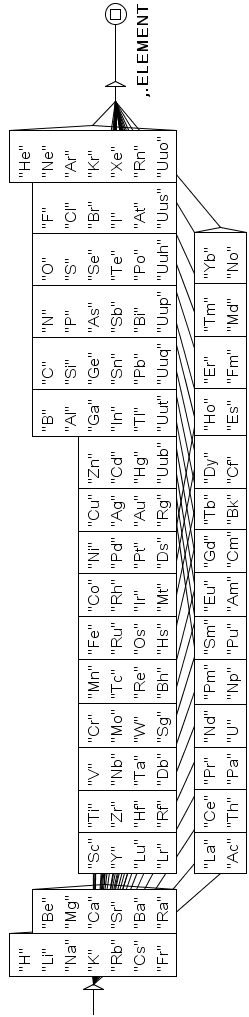
\includegraphics[height=24cm]{resources/img/fig3-12.png}
\caption{Graphe-dictionnaire des éléments chimiques\label{elements}}
\end{center}
\end{figure}

\bigskip
\noindent La figure \ref{elements} montre un graphe reconnaissant les symboles chimiques. On peut
voir sur cette figure un premier avantage par rapport aux dictionnaires compressés : l’utilisation
des guillemets permet de forcer le respect de la casse. Ainsi, ce graphe reconnaîtra bien \verb+Fe+
mais pas \verb+FE+, alors qu’il est impossible de spécifier une telle interdiction dans un DELAF
usuel.

\bigskip
\noindent Le second avantage des graphes-dictionnaires est qu’ils peuvent exploiter les résultats
fournis par les dictionnaires appliqués précédemment. Ainsi, on peut appliquer le dictionnaire
général, puis étiqueter comme noms propres les mots inconnus commençant par une majuscule à l’aide
du graphe \verb$NPr+$ de la figure~\ref{graph-NPr}. Le \verb$+$ dans le nom du graphe lui donne une
priorité basse afin qu’il soit appliqué après le dictionnaire général. Pour fonctionner, ce graphe
se base sur les mots qui sont toujours inconnus après le passage du dictionnaire général. Les
crochets correspondent à une définition de contexte (voir la section \ref{section-contexts}).

\begin{figure}[!ht]
\begin{center}
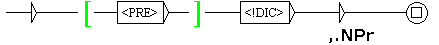
\includegraphics[width=10.5cm]{resources/img/fig3-13_fr.png}
\caption{Graphe-dictionnaire étiquetant comme noms propres les mots inconnus commençant par une
majuscule
\label{graph-NPr}}
\end{center}
\end{figure}

\bigskip
\noindent Comme les graphes-dictionnaires sont appliqués par le moteur du programme \verb+Locate+,
ils peuvent utiliser tout ce que le programme \verb+Locate+ autorise. En particulier, il est
possible d’utiliser les filtres morphologiques\index{Filtre morphologique} (section~\ref{section-filters}) et le mode morphologique (section~\ref{section-morphological-mode}).\index{Mode
morphologique}
Ainsi, le graphe de la figure \ref{graph-CR} utilise ces filtres pour reconnaître les nombres en
chiffres romains. Notons qu’il utilise également des contextes afin d’éviter, par exemple, que
\verb+C+ ne soit pris comme chiffre romain quand il est suivi par une apostrophe.

\begin{figure}[!p]
\begin{center}
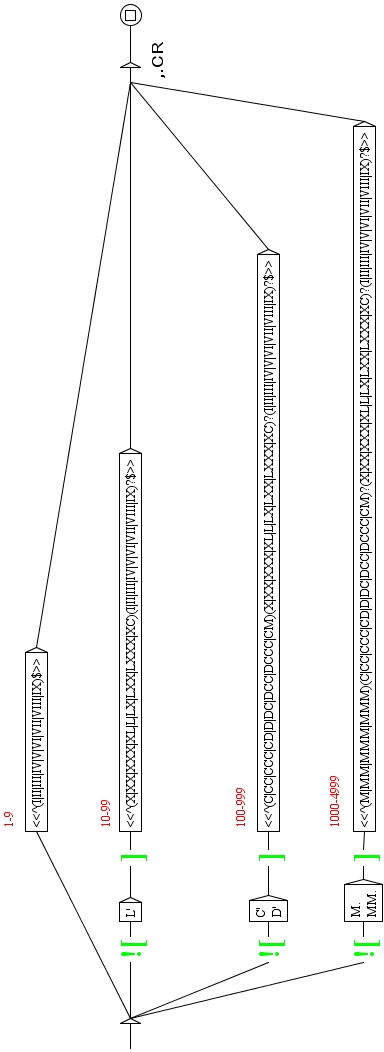
\includegraphics[height=24cm]{resources/img/fig3-14.png}
\caption{Graphe-dictionnaire reconnaissant les nombres en chiffres romains\label{graph-CR}}
\end{center}
\end{figure}

\bigskip
\noindent Par défaut, les graphes-dictionnaires sont appliqués en mode MERGE. Il est possible 
de les appliquer en mode REPLACE, en ajoutant à leur le nom le suffixe \verb+-r+. Celui-ci se
combine avec les priorités \verb-+- et \verb+-+:

\bigskip
\verb?bagpipe-r.fst2  McAdam-r-.fst2  phtirius-r+.fst2?


\subsubsection{Exporter les entrées produites comme dictionnaire du mode morphologique}
\index{Dictionnaire!du mode morphologique}
Les entrées produites par un graphe-dictionnaire sont consultées
par le programme \verb+Locate+ quand il rencontre des masques lexicaux qui nécessitent la consultation
d'un dictionnaire.

\bigskip
\noindent Cependant, cette fonctionnalité est restreinte quand le masque lexical est en mode morphologique
(cf.~section~\ref{section-morphological-mode}). On ne peut pas déclarer un graphe-dictionnaire
comme dictionnaire du mode morphologique de la manière habituelle (cf.~section~\ref{dic-mode-morpho}),
car ce n'est pas un fichier \verb+.bin+. Quand on est en mode morphologique, les masques
lexicaux qui nécessitent la consultation d'un dictionnaire ne déclenchent pas la consultation
de graphes-dictionnaires. En compensation, on dispose de plusieurs solutions.
\begin{itemize}
\item On peut envisager d'invoquer le graphe-dictionnaire depuis la partie du graphe qui est en mode morphologique.
\item Unitex produit de façon interne un dictionnaire des formes reconnues dans le texte par un
graphe-dictionnaire. Si le nom du graphe-dictionnaire contient l'option \verb+b+ (voir ci-dessous
Conventions de nommage), ce dictionnaire produit automatiquement est inclus implicitement parmi
les dictionnaires du mode morphologique, de telle sorte qu'il est consulté quand le programme
 \verb+Locate+ rencontre des masques lexicaux en mode morphologique. Mais cette solution 
 ne fonctionne que pour les formes reconnues par le graphe-dictionnaire pendant l'application initiale
 des dictionnaires (cf.~section~\ref{section-applying-dictionaries}), et non pour celles qui n'apparaissent
 dans le texte que comme parties de tokens.
\end{itemize}
Si on ajoute \verb+z+ à la place de  \verb+b+, le dictionnaire produit de façon interne pour le texte est immédiatement
compressé, et il peut être consulté quand d'autres graphes-dictionnaires sont appliqués  par la suite.
 
\subsubsection{Conventions de nommage}
Le processus de nommage d'un graphe-dictionnaire s'établit comme suit :\\

\verb$nom(-XYZ)([-+]).fst2$\\

\noindent où:
\begin{itemize}
\item \verb+X+ prend l'une des valeurs \verb+[rRmM]+: \verb+r+ signifie mode REPLACE; \verb+M+
signifie mode MERGE (mode par défaut);
\item \verb+Y+ prend l'une des valeurs \verb+[bBzZ]+: option qui régit la construction d'un
dictionnaire du mode morphologique (voir ci-dessus);
\item \verb+Z+ prend l'une des valeurs \verb+[aAlLsS]+: \verb+a+ signifie que le graphe est appliqué
en mode "All matches"; \verb+l+ signifie mode "Longest matches" (mode par défault); 
\verb+s+ signifie "Shortest matches".
\end{itemize}


\subsection{Graphe-dictionnaire morphologique}
\label{section-morphological-dictionary-graphs}\index{Graphe-dictionnaire!morphologique}
Dans un graphe-dictionnaire, chaque chemin doit, par défaut, produire une entrée lexicale à inclure dans le dictionnaire du
texte. Dans un graphe-dictionnaire morphologique, chaque chemin doit produire une séquence d'une ou plusieurs
étiquettes délimitées par des accolades et conformes à la syntaxe des lignes du DELAF
 (section~\ref{section-DELAF-entry-syntax}).
Les sorties de tels graphes seront utilisées comme entrées pour construire l'automate du texte. Nous
les appelons ``graphes-dictionnaires morphologiques'' parce que leur principale utilité est de
fournir de nouvelles analyses morphologiques dans l'automate du texte, grâce au mode morphologique
(voir \ref{section-morphological-mode}). Cette fonctionnalité est utile pour des langues
agglutinantes comme le coréen.
Pour pouvoir utiliser un graphe comme graphe-dictionnaire morphologique, on le déclare
par une barre oblique (slash, /) comme premier caractère de sa sortie, comme dans la figure \ref{morphoA}.

\begin{figure}[!ht]
\begin{center}
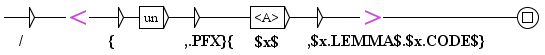
\includegraphics[width=14cm]{resources/img/fig3-14a.png}
\caption{Exemple de graphe-dictionnaire morphologique\label{morphoA}}
\end{center}
\end{figure}

\noindent La règle est simple: toute sortie du graphe-dictionnaire commençant par une barre oblique (slash, /) 
est ajoutée au fichier \verb+tags.ind+, \index{\verbc{tags.ind}} situé dans le répertoire du texte.
Ce fichier est utilisé par le programme \verb+Txt2Fst2+ afin d'ajouter des interprétations à
l'automate du texte. La grammaire de la figure \ref{morphoA} reconnaît des mots
formés par le préfixe \verb+un+ suivi d'un adjectif. Si on l'applique comme graphe-dictionnaire,
on obtient de nouveaux chemins dans l'automate du texte comme le montre la figure
\ref{morphoB}. Remarquons que lorsque deux tags correspondent à des analyses dans la même unité lexicale, le lien entre eux est affiché par une ligne discontinue.

\begin{figure}[!ht]
\begin{center}
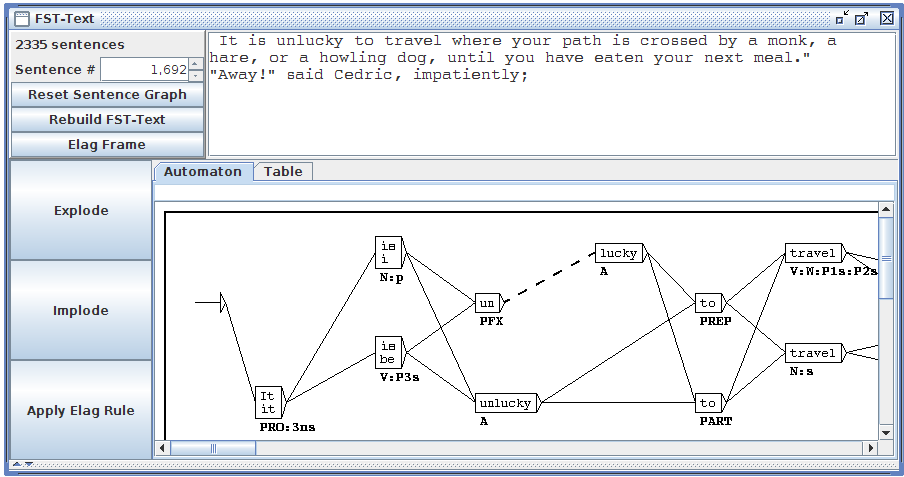
\includegraphics[width=15cm]{resources/img/fig3-14b.png}
\caption{Chemin ajouté par un graphe-dictionnaire morphologique\label{morphoB}}
\end{center}
\end{figure}

\section{Bibliographie}

Le tableau ~\ref{ref-dicos} donne quelques références relatives aux dictionnaires électroniques de
mots simples et composés. Pour plus de détails, consultez la page de références sur le site
web d’Unitex: \url{http://www-igm.univ-mlv.fr/~unitex}

\bigskip
\begin{table}[!ht]
\begin{center}
\begin{tabular}{|l|c|c|}
\hline
\textbf{Langue} & \textbf{Mots simples} & \textbf{Mots composés} \\
\hline
English & \cite{klarsfeld}, \cite{monceaux-1995} & \cite{delac-anglais},
\cite{these-Savary} \\
\hline
French & \cite{formes-ambigues}, \cite{dicos-francais}, \cite{jacques-1995} & \cite{dicos-francais},
\cite{Gross96},
\cite{max-1993},
\cite{syntaxe-de-ladverbe} \\
\hline
Modern Greek & \cite{modern-greek}, \cite{matthieu-anastasia}, \cite{these-tita} & \cite{tita-2002},
\cite{anastasia-2002} \\
\hline
Italian & \cite{delaf-italien}, \cite{delaf-italien-book} & \cite{composes-italien} \\
\hline
Spanish & \cite{blanco-2000} & \cite{blanco-1997} \\
\hline
Portuguese & \cite{eleuterio1995}, \cite{ranchhod1996b}, \cite{ranchhodd1998},
\cite{muniz2005} & \cite{ranchhod1991}, \cite{ranchhodd1998} \\
\hline
\end{tabular}
\caption{Quelques références bibliographiques sur les dictionnaires électroniques\label{ref-dicos}}
\end{center}
\end{table}
